\documentclass[fleqn,usenatbib]{rasti}

\usepackage[T1]{fontenc}
\usepackage{newtxtext,newtxmath}
\usepackage{graphicx}
\usepackage{amsmath}
\usepackage{booktabs}
\usepackage{array}
\usepackage{multirow}
\usepackage{longtable}
\usepackage{multicol}
\usepackage{siunitx}
\usepackage{placeins}
\usepackage{flushend}
\usepackage{lastpage}
\hypersetup{hypertexnames=false}

\graphicspath{{./}}
\newcolumntype{L}[1]{>{\raggedright\arraybackslash}p{#1}}

\title[Linear-probe diagnostics of source injection]{Linear-probe diagnostics
of observed and source-injected strong-lens images in DESI Legacy Imaging
Surveys DR10}

\author[Balaji \& Johnson]{
Aditrivaishnavi~Balaji,$^{1}$\thanks{E-mail: aditrivaishnavi@gmail.com}
and Parker~T.~Johnson$^{2}$
\\
$^{1}$BASIS Independent Silicon Valley, 1290 Parkmoor Ave, San Jose, CA
95126, USA\\
$^{2}$Steward Observatory, The University of Arizona, 933 North Cherry
Avenue, Tucson, AZ 85721, USA
}

\date{}
\pubyear{2026}

\begin{document}
\label{firstpage}
\pagerange{\pageref{firstpage}--\pageref{LastPage}}
\maketitle

\begin{abstract}
Injection--recovery characterizes CNN strong-lens finders, but its
interpretation depends on the simulated images presented to the detector. For
a frozen EfficientNetV2-S trained on DESI Legacy Imaging Surveys DR10 cutouts,
we measure conditional recovery and observed--injected distinguishability
separately. Matched and paired controls identify differences already present
before source insertion and measure detector responses to specified
construction changes. Dependency-aware linear probes compare four
representations---the operational detector's pooled penultimate features,
self-supervised survey features, ImageNet features, and pixel statistics---for
43 selected observed systems and 6,336 source-injected images.
The populations separate in all four representations, with out-of-fold
receiver-operating-characteristic AUCs of 0.991, 0.958, 0.979, and 0.981,
respectively. A leading pixel-statistic offset is already present between
observed systems and bare targets. Along a separately fitted operational
observed--bare axis, the mean injection movement is near zero despite
heterogeneous pairwise effects. Separately, the finder recovers 3.45 per cent
of a 49,500-scene grid with no visibility cut. Modelled source-photon sampling
lowers recovery, whereas the single-S\'{e}rsic construction is recovered more
often than its paired structured-source counterpart. On 43 fixed targets,
expectation-image recovery varies non-monotonically with source brightness and
peaks at 18.6 per cent.
Together, these analyses reveal differences between the selected populations
within the actual finder, identify a pre-insertion offset, and measure
responses to controlled injection choices. They provide a practical basis for
comparing future injection pipelines using trained finders.
\end{abstract}


\begin{keywords}
gravitational lensing: strong -- surveys -- techniques: image processing --
Data Methods -- Machine Learning
\end{keywords}

\section{Introduction}

Strong gravitational lenses constrain galaxy mass profiles, dark-matter
structure, and cosmological distances \citep[e.g.][]{Treu2010,Collett2015}.
Building large samples requires scalable discovery methods, including
convolutional neural networks (CNNs). Population inference also requires a
selection function: a model of whether a lens is physically detectable and
whether a specified search procedure finds it
\citep{Sonnenfeld2023,Sonnenfeld2024}. Injection--recovery measures the
response after synthetic lensed light is added to survey images. Without a
separate detectability condition, its recovery fraction combines physical
visibility with finder response.

CNN lens finders perform well on simulated benchmarks and labelled
observational samples \citep[e.g.][]{Petrillo2017,Lanusse2018,Jacobs2019,
Canameras2021,Storfer2024}, but their calibration depends on the simulations
used. Some pipelines inject parametric S\'{e}rsic sources lensed by idealised
mass models \citep[e.g.][]{Herle2024}; others use images of observed galaxies
as source-plane templates \citep[e.g.][]{Canameras2021,Rojas2022,Schuldt2023}.
Cross-pipeline results combine differences in target selection, lens models,
source distributions, image processing, and source structure
\citep{Jaelani2024,Canameras2024}. A classifier two-sample test
asks whether a model can tell which of two samples an object came from using
only a chosen representation \citep{LopezPazOquab2017}. In strong-lens work,
self-supervised survey representations have supported lens discovery
\citep{Stein2022}, while domain-adaptation methods have explicitly addressed
differences between simulated and observed lens data \citep{Parul2025}.
A linear probe is an \(L_2\)-regularised logistic regression fitted to frozen
features; its receiver-operating-characteristic area under the curve (AUC)
measures how well the two samples are separated on held-out data.

Injection recovery measures how often a finder responds to a specified
simulated population. A complementary representation-level comparison asks
how clearly observed and injected populations separate in a chosen feature
space. We therefore use a linear probe of the operational detector's pooled
penultimate features as a detector-specific diagnostic. It reuses the trained
representation to evaluate a held-out observed--injected readout for the fixed
finder. We
apply the same dependency-aware procedure to self-supervised survey features,
generic ImageNet features, and elementary pixel statistics to map how broadly
separation appears across representations. Comparing the four protocols shows
whether separation is specific to the lens-trained network or also appears in
unrelated learned and pixel-level representations.

We interpret the comparison using the existing lens-classification score,
native-pixel summaries, and matched observed--bare--injected controls.
We also measure how the fixed detector responds to the injection grid,
source-photon sampling, source construction, and source brightness. Together,
these analyses distinguish
population-level representation differences from responses to controlled
construction choices.

\section{Data, samples, and detector}
\label{sec:data_detector}

We use DR10 cutouts to measure injection recovery and feature-space
differences between the observed and simulated samples.

\subsection{DESI Legacy Imaging Surveys DR10}
\label{sec:dr10_data}

We use $g$-, $r$-, and $z$-band coadded imaging from the tenth data release
(DR10) of the DESI Legacy Imaging Surveys \citep{Dey2019}.\footnote{DR10
description: \url{https://www.legacysurvey.org/dr10/description/}, accessed
29 August 2026.} The images have a
pixel scale of $0.262\;\mathrm{arcsec\;pixel^{-1}}$, and the nominal
$5\sigma$ point-source depths of the Legacy Surveys are $g \approx 24.7$,
$r \approx 23.9$, and $z \approx 23.0$~mag (AB). Because the delivered
point-spread function (PSF) and depth vary across the footprint and affect the
detectability of lensed features, these nominal depths characterise the survey
design rather than every location in DR10. Where these quantities enter the
injection experiments, we therefore use the local catalogue measurements at
each injection-target position rather than assigning one survey-wide value.

The Tractor catalogue is the model-based source catalogue produced from the
Legacy Surveys imaging \citep{Lang2016,Dey2019}.\footnote{DR10 catalogue
documentation: \url{https://www.legacysurvey.org/dr10/catalogs/}, accessed
29 August 2026.} For each catalogue object used in this
study, we extract a $101 \times 101$ pixel cutout
($26.5 \times 26.5\;\mathrm{arcsec}^{2}$) centred on its Tractor position.
Cutouts are stored in nanomaggies, for which the AB zeropoint is 22.5, and the
$g$, $r$, and $z$ images form the three detector input channels; no other DR10
catalogue or imaging products are used as detector inputs in this analysis.

\subsection{Preprocessing}
\label{sec:preprocessing}

We apply the same preprocessing to observed and injected cutouts. For each
band $b$, let $A$ denote the annulus containing pixels whose radial distance
from the cutout centre satisfies $20 \leq r < 32$ pixels. We define
\begin{equation}
 m_b = \operatorname{median}_{i \in A}(x_{b,i}), \qquad
 s_b = \operatorname{median}_{i \in A}\lvert x_{b,i}-m_b\rvert + 10^{-8},
\end{equation}
and transform each pixel as
\begin{equation}
 x'_{b,i} =
 \operatorname{clip}\left(\frac{x_{b,i}-m_b}{s_b},-10,+10\right).
\label{eq:raw_robust}
\end{equation}
Thus, each band is centred and scaled using a robust local reference while
preserving the full $101 \times 101$ field. The scale \(s_b\) is the unscaled
median absolute deviation (MAD), rather than a Gaussian-equivalent standard
deviation.

All detector comparisons retain the $20$--$32$ pixel normalisation annulus
used during training. The annulus can contain light from the central object or
injected source, so its median and MAD can depend on astrophysical structure
as well as the local background. These statistics define the detector's
trained input mapping.

\subsection{Detector development and evaluation roles}
\label{sec:data_roles_overview}

Table~\ref{tab:detector_roles_overview} summarizes the samples used for
training, validation, threshold calibration, and evaluation. Development
positives are noisy labels from the literature-reviewed candidate set and the
lower-confidence catalogue-candidate set; confirmed lenses are reserved for
evaluation. False-positive rate (FPR) denotes the fraction of catalogue-negative
examples at or above threshold. We calibrate the threshold
on one negative sample and estimate its FPR on another.

\begin{table*}
\caption{Detector-development and evaluation roles. ``Reviewed candidates''
are Lenscat systems classified as candidates---rather than confirmed lenses,
non-lenses, or uncertain systems---after object-level review of the published
evidence.
``Additional catalogue candidates'' are lower-confidence catalogue records
used only as noisy positive examples. The calibration, achieved-FPR, and
selected-system samples are disjoint and are used only after training.}
\label{tab:detector_roles_overview}
\centering
{\small
\setlength{\tabcolsep}{4pt}
\begin{tabular}{L{0.21\textwidth}rL{0.29\textwidth}L{0.27\textwidth}}
\toprule
Role & Negative examples & Positive or observed examples & Function \\
\midrule
Training: reviewed + additional &
286\,679 & 238 reviewed candidates + 3\,395 additional catalogue candidates &
Primary training set; 290\,312 rows \\
Validation: reviewed + additional &
61\,437 & 64 reviewed candidates + 714 additional catalogue candidates &
Development diagnostics and sensitivity-checkpoint selection; 62\,215 rows \\
Training: reviewed candidates only &
286\,679 & 238 reviewed candidates &
Alternative positive-label composition; 286\,917 rows \\
Validation: reviewed candidates only &
61\,437 & 64 reviewed candidates &
Checkpoint selection for the corresponding runs; 61\,501 rows \\
Full test partition &
61\,435 & 63 confirmed systems &
Source partition for final evaluation roles \\
Threshold calibration &
20\,002 & None &
Set the primary or checkpoint-specific operating threshold \\
Achieved-FPR evaluation &
12\,512 & None &
Evaluate catalogue-negative threshold exceedance \\
Selected-system evaluation &
None & 43 confirmed systems &
Recovery among the 43 selected confirmed systems \\
Exploratory-analysis-development role &
None & 20 confirmed systems &
Excluded from endpoint and observed-reference denominators \\
\bottomrule
\end{tabular}
}
\end{table*}

\subsection{Labelled samples and provenance}
\label{sec:sample_provenance}

Lenscat v1.1.3 is the public, community-contributed strong-lens catalogue
compiled by \citet{Vujeva2025} and archived by \citet{LenscatV113}.

The positive parent catalogue was assembled from Lenscat. We selected
5,104 entries whose names identified them with DESI imaging; 4,788 were
associated with a Tractor source in the processed DR10 sweeps within
5~arcsec. Lenscat places 389 of these systems in its highest-confidence
category and 4,399 in a lower-confidence candidate category. All 389
highest-confidence records underwent object-level literature review. The
4,399 lower-confidence records supplied noisy positive labels for detector
development, subject to the role exclusions in
Section~\ref{sec:training_sets}. Lenscat
confidence was not treated as confirmation because its highest category can
denote either spectroscopically confirmed multiple images or the highest grade
assigned by a contributing study \citep{Vujeva2025}. The entries originate from heterogeneous
discovery samples, including the DESI Legacy Imaging Surveys searches of
\citet{Huang2020,Huang2021}, \citet{Stein2022}, and \citet{Storfer2024}.

Literature review identified 63 confirmed lenses among the 389 reviewed
systems. Of these, 50 have secure spectroscopic redshifts for both deflector
and source, seven have secure lens evidence but incomplete or
lower-confidence spectroscopy, and six are confirmed by imaging or lens
modelling without secure redshifts for both components. The available
literature provides heterogeneous spectroscopic and imaging support across
the cohort. The four non-lenses and two uncertain systems are excluded from
lens-performance estimates; the remaining 320 candidates form the reviewed
source of noisy positive labels for detector development. For the 43-system
evaluation cohort, object-level confirmation evidence and available
deflector and source redshifts are listed in Appendix
Table~\ref{tab:confirmed_43_provenance}.

\begin{table}
\caption{Literature-based classifications for the 389 reviewed Lenscat
records.}
\label{tab:evidence_review_status}
\centering
\begin{tabular}{lr}
\toprule
Scientific status & Number \\
\midrule
Confirmed lens & 63 \\
Candidate & 320 \\
Confirmed non-lens & 4 \\
Uncertain & 2 \\
\midrule
Total & 389 \\
\bottomrule
\end{tabular}
\end{table}

The negative parent sample was drawn from the Tractor catalogue in two stages.
The sampling frame required finite coordinates,
$-18^\circ < \delta < +32^\circ$, a Tractor morphological type of SER, DEV,
or REX, at least three exposures in each of \(g,r,z\), and none of mask bits
1, 5, 6, 7, 11, 12, or 13. It also required a separation of at least
11~arcsec from the 5,104-entry DESI-named Lenscat parent catalogue. For rows
with positive fitted \(z\)-band flux, the observed magnitude, not corrected
for Galactic foreground extinction, had to satisfy \(z<20\). Rows with
finite non-positive \(z\)-band flux have no logarithmic magnitude and were
therefore retained without the \(z<20\) requirement; the available records do
not document a scientific reason for this exemption. Colour was not an
eligibility cut, but \(g-r\) contributed to the sampling strata described
below. All reported analyses use this fixed sample. The available sampled-row
table retains the \(z\)-band exposure count but omits the corresponding
\(g\)- and \(r\) columns. The archived roster and image cutouts are sufficient
to reproduce the reported analyses, but the available table does not contain
the \(g\)- and \(r\)-band exposure counts needed to recheck those two
eligibility criteria row by row.

Rows in the sampling frame were assigned to two sampling strata. \(N1\)
contains the remaining candidates; \(N2\) uses proxies for lens-like negative
morphology and is assigned by the first matching condition: DEV type with
\(r\)-band flux at least 5~nmgy; SER or DEV type
with Tractor \(\mathtt{shape\_r}\geq1.8\)~arcsec;
\(g-r\leq0.4\) and \(r\leq20.5\)~mag; or
\(\mathtt{shape\_r}\geq2.0\)~arcsec and \(r\)-band flux at least 3~nmgy.
These proxies stratify sampling; they are not eligibility cuts and do not use
detector scores. Within exposure-count and Tractor-type strata, the procedure
targeted an 85:15 \(N1:N2\) sample before final eligibility filtering.

The sampler drew 453,100 rows. Of these, 6,207 lacked a final cutout, leaving
446,893 rows with usable pixels. The final negative pool additionally
required finite \(g,r,z\) photometry and removed any row within 11~arcsec of a
Lenscat system or catalogue-positive centre. A total of 37,342 usable-cutout
rows failed at least one of these final photometry or proximity rules.
The retained pool therefore contains 409,551 catalogue-negative rows:
343,469 in \(N1\) and 66,082 in \(N2\). The final stratum proportions need not
equal the sampling target because eligibility was applied after sampling.
These are catalogue negatives, not individually verified non-lenses.

The positive and negative parent samples were not selected under identical
eligibility rules. In particular, the magnitude, morphology, exposure, mask,
and declination restrictions above were not applied to the positive
catalogue. Eight of the 63 confirmed lenses, and 2,291 of all 4,788
catalogue-positive rows, lie outside the negative sample's declination
window. The observed--injected comparison therefore includes differences in
deflector populations and survey conditions alongside source insertion.

\subsection{Development and test partitions}
\label{sec:data_partitions}

The clean sample contains 409,551 negatives and 63 confirmed lenses. Before
noisy candidate labels are added, the grouped split assigns 286,679 negatives
to training, 61,437 to validation, and 61,435 to test; all 63 confirmed lenses
are assigned to test before model development. No noisy candidate label is
counted as confirmed.

Rows were grouped by object identity, sky proximity, overlapping cutouts,
NSIDE$=128$ NESTED HEALPix cell \citep{Gorski2005}, and known physical system
before partitioning. These grouping rules keep objects linked by the recorded
identities and spatial or physical-system information within the same
partition. Candidate labels were added under the same grouping rules.

Before detector scoring, disjoint spatial groups supplied 20,002 negatives
for threshold calibration and 12,512 for false-positive-rate evaluation. The
63 confirmed systems were excluded from detector fitting, validation,
checkpoint selection, and threshold calibration. Twenty had an exploratory
feature-analysis-development role and are excluded from all final endpoint and
observed-reference denominators. The published roster of the remaining 43
systems defines the selected-system endpoint and the observed-reference
sample. We do not have a documented general scientific eligibility rule that
independently selects those 43 from all 63 confirmed systems. The 43-system
roster was not chosen using detector scores.
No development object shares a recorded identity or physical group with the
calibration, evaluation, or injection samples. Where a spatial-component
identifier is available, it also shows no shared component; the calibration,
achieved-FPR, and injection-target samples additionally have no flagged
development HEALPix or 38-arcsec contact. The available identities, group
labels, and sky-neighbour checks show no recorded overlap between development
and evaluation samples. Exact footprint polygons are unavailable for part of
the development set, so broader geometric overlap cannot be tested. The
selected-system recovery fraction is a finite-cohort summary of these 43
heterogeneous systems.

\subsection{Positive examples and training-set composition}
\label{sec:training_sets}

Because the clean training and validation partitions contain no confirmed
positive examples, detector training uses noisy catalogue-positive labels.
The 320 objects assigned candidate status after literature review provide one
source of positive examples; the 4,399 lower-confidence catalogue candidates
provide an additional source. Rows spatially linked to the test partition are
excluded before the development sets are formed. This removes 18 reviewed
candidates and 290 additional catalogue candidates.

The primary training set combines reviewed and additional catalogue candidates;
the comparison set uses reviewed candidates only, with the same negatives
(Table~\ref{tab:detector_roles_overview}). Their training negative-to-positive
ratios are approximately \(79{:}1\) and \(1205{:}1\), respectively. Confirmed
lenses, confirmed non-lenses, and uncertain systems enter neither composition.

Both positive-example sets contain candidate labels rather than uniform
confirmed truth; the contamination fraction of the additional catalogue
candidates has not been measured.
In natural-prevalence runs, training rows are shuffled and sampled without
replacement each epoch, with the incomplete final mini-batch omitted; the
loss is unweighted binary cross-entropy. Accuracy is not used for checkpoint
selection or operating point assessment because an all-negative classifier
would be favoured by the class imbalance while recovering no labelled
positives.

\subsection{Primary detector protocol}
\label{sec:detector_training}

The finder is an ImageNet-initialised EfficientNetV2-S with a binary output
\citep{Deng2009,Russakovsky2015,TanLe2021}, subsequently trained for lens
classification. ImageNet-1K is a labelled natural-image dataset whose pretrained
weights supply a general visual initialization. The trained finder's pooled
representation and the distinct external feature protocols are defined in
Section~\ref{sec:linear_probe_methods}.

The primary run uses reviewed and additional catalogue candidates, seed 42,
natural-prevalence sampling, and a cosine learning-rate schedule. It trains
for 160 epochs with AdamW, a five-epoch learning-rate warm-up, and the
backbone frozen for the first five epochs. The initial learning rate is
\(3.88\times10^{-4}\), and weight decay is \(10^{-4}\). Training uses
mixed-precision forward passes, micro-batches of 64 accumulated to an
effective batch size of 512, and omits the incomplete final mini-batch. Early
stopping is disabled.
Horizontal and vertical flips are applied independently with probability 0.5,
followed by a rotation selected uniformly from $0^\circ$, $90^\circ$,
$180^\circ$, and $270^\circ$. We use no colour or noise augmentation.

The primary detector is the epoch-160 checkpoint; validation, calibration,
and evaluation scores do not select it. All primary-detector evaluations use the same
preprocessing and operating threshold defined in
Section~\ref{sec:scoring_contract}.

\subsection{Detector-sensitivity training panel}
\label{sec:checkpoint_panel_design}

The sensitivity panel contains 12 EfficientNetV2-S runs that share the
primary architecture and training duration but vary the positive sample,
random seed, sampler, or learning-rate schedule:
\begin{itemize}
\item six baseline runs cross the two positive-example sets---reviewed
candidates only, or reviewed plus additional catalogue candidates---with
seeds 42, 123, and 2026 under natural-prevalence sampling and cosine
scheduling;
\item two sampler runs use seed 42 and seeded 50:50 class-balanced
weighted sampling with replacement for the two positive-example sets;
\item two schedule runs use seed 42 and natural-prevalence sampling for the
two positive-example sets, with a step schedule that halves the learning rate after epoch
130 instead of cosine decay; and
\item two additional runs use reviewed candidates only, with seeds 7 and 2027
under the baseline sampler and schedule.
\end{itemize}
The repeated seeds probe sensitivity to training stochasticity; they are not a
statistical sample of all possible trained models. Sampler and schedule pairs
change one training choice at seed 42. Changing the positive sample also
changes its composition, prevalence, and size; that comparison measures
detector sensitivity to the combined change.

For each sensitivity run, we select the checkpoint with the highest validation
average precision; selected epochs range from 17 to 103. These checkpoints
form a secondary analysis; the epoch-160 checkpoint remains the primary
detector.
Appendix~\ref{app:checkpoint_sensitivity} reports the complete panel.

Figure~\ref{fig:data_training_flow} summarizes the sample, training, and
evaluation roles.

\begin{figure*}
\centering
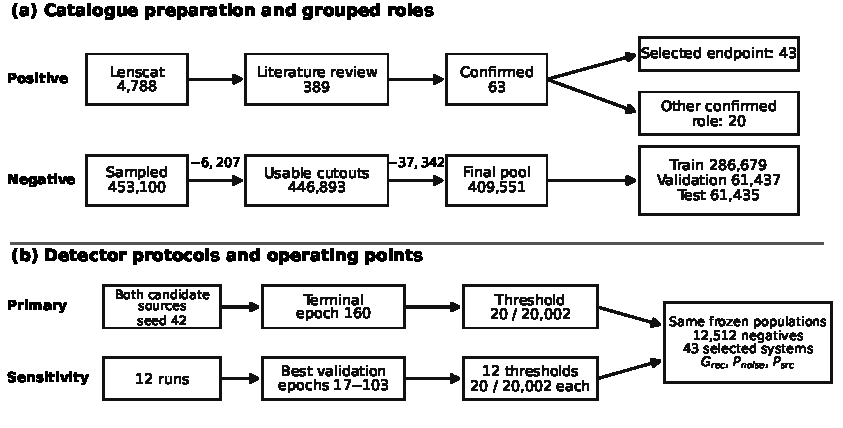
\includegraphics[width=\textwidth]{figures/section2_data_training_flow.pdf}
\caption{Data preparation, detector training, and evaluation roles. Panel A
shows the catalogue-positive evidence review and the negative-sample flow
before grouped train, validation, and test assignment. Panel B separates the
primary terminal-epoch protocol from the 12-run validation-selected
sensitivity panel. The primary detector and each sensitivity checkpoint use
the same 20,002-row calibration population. Each model is calibrated
independently by choosing the threshold with 20 exceedances, then evaluated
on the same corresponding held-out cohorts. The primary uses reviewed and
additional catalogue candidates. The sensitivity panel includes both
positive-sample compositions and the specified sampler, schedule and seed
variants. Arrows show data or model flow; evaluation does not feed back into
training.}
\label{fig:data_training_flow}
\par\smallskip{\raggedright\noindent\textit{Alt text:} Two linked flow diagrams. The first
tracks catalogue positives to 63 confirmed systems and tracks 453,100 sampled
negatives to 409,551 retained rows and grouped data partitions. The second
shows noisy-label training sets feeding the primary epoch-160 detector and a
12-run sensitivity panel, followed by separate calibration thresholds and
the same held-out evaluation samples.\par}
\end{figure*}

\section{Injection models and experiment sets}
\label{sec:injection_models}

\subsection{Overview of simulation and control sets}
\label{sec:simulation_inventory}

We use \emph{deflector} for the foreground lens galaxy in an observed strong
lens and \emph{injection target} for a catalogue galaxy into whose observed
DR10 cutout a simulated lensed source is inserted.
The source family, injection-target population, parameter distribution, noise
treatment, detector, and operating threshold are distinct design axes that can
differ between experiments.
Table~\ref{tab:simulation_sets} summarizes each experiment's question,
population, image construction, and analysis role. Source, target, noise, and
detector settings are specified separately for each experiment. Below,
signal-to-noise ratio is abbreviated as S/N and false-positive rate as FPR. We write
\(p=\operatorname{sigmoid}(\ell)\) for display of a detector's single output
logit \(\ell\); \(p\) is not assumed to be a calibrated probability.

\begin{table*}
\caption{Simulation and control sets used in the study. The visibility
column states the admission policy; absence of an independent visibility cut
retains low-signal configurations. Derived and paired samples reuse the
targets, sources, and scene components indicated in the table.}
\label{tab:simulation_sets}
\centering
{\small
\setlength{\tabcolsep}{2.5pt}
\begin{tabular}{L{0.10\textwidth}L{0.18\textwidth}L{0.20\textwidth}L{0.14\textwidth}L{0.16\textwidth}L{0.15\textwidth}}
\toprule
ID & Question & Source and injection targets & Size & Visibility policy & Analysis role \\
\midrule
$G_{\rm rec}$ &
How often does the primary detector respond over the fixed radius and
observing-condition grid? &
Single S\'{e}rsic sources in catalogue-negative injection targets; source and
lens nuisance draws are shared over radius &
49\,500 injections; 4\,500 distinct targets; nine cells &
No independent S/N or visibility cut &
Fixed-detector recovery and radius curve \\

$G_{\rm domain}$ &
Can the selected observed and injection populations be separated in a fixed
representation? &
Massive-early-type subset of \(G_{\rm rec}\), compared with the 43
selected confirmed systems &
6\,336 injections in 576 targets plus 43 observed systems &
Inherited from \(G_{\rm rec}\) &
Dependency-grouped finite-cohort separation \\

$G_{\rm match}$ &
How does a fixed injection move a matched target along an observed--bare
feature axis? &
Each of the same 43 observed systems and one score-blind matched
\(G_{\rm rec}\) target, using its bare cutout and corresponding
\(\theta_{\rm E}=1.5\)-arcsec injected image &
43 triplets (129 rows) in 43 dependency components &
No post-render selection or target-flux floor &
Cross-fitted representation-axis movement \\

$P_{\rm noise}$ &
How does modelled source-photon sampling change primary-detector response? &
Each \(G_{\rm rec}\) source expectation and eight
\(g=150\ {\rm e^{-}\,nmgy^{-1}}\) Poisson realizations on the same target &
49\,500 deterministic expectation scenes and 396\,000 photon-draw
realizations &
Inherited from \(G_{\rm rec}\); no independent S/N cut &
Photon-minus-expectation paired risk difference \\

$P_{\rm src}$ &
How does the declared structured source construction compare with its
single-S\'{e}rsic twin? &
Restricted high-S/N COSMOS F814W constructions and deterministic catalogue
S\'{e}rsic twins paired on the same \(G_{\rm rec}\) target, with a distinct
target for each pair &
1\,584 pairs; eight draws per pair; 12\,672 paired draw comparisons
(25\,344 arm rows) &
Source-quality restrictions only; no post-render S/N or score cut &
Photon-averaged paired risk difference \\

$C_{\rm bright}$ &
How does response vary with source brightness and photon realization? &
The 43 \(G_{\rm match}\) targets with their stored 1.5-arcsec isolated source
expectations, rescaled to eight magnitudes &
3\,096 derived images and training-preprocessing scores &
No visibility cut; fixed target and geometry &
Fixed-target brightness and source-photon response \\
\bottomrule
\end{tabular}
}
\end{table*}

The recovery set \(G_{\rm rec}\) spans 11 Einstein radii from 0.5 to
3.0~arcsec in 0.25-arcsec steps. Its nine retained \(r\)-band PSF--depth
cells each contain 500 distinct targets, and every target is rendered at all
11 radii. Source, lens-nuisance, colour, and normalized source-offset draws
are shared across radii; only \(\theta_{\rm E}\) and the corresponding
physical source offset vary. The PSF and depth values define descriptive
strata, not interventions.

The experiment retains configurations across the full grid without a
signal-to-noise or visibility threshold, allowing both recovery and failure
to contribute to the conditional response. Population weighting would require
an external distribution over the retained cells.

\(G_{\rm domain}\) reuses a \(G_{\rm rec}\) subset, while \(G_{\rm match}\)
reuses one target's bare and 1.5-arcsec injected pixels per reference. The
primary detector endpoints and \(G_{\rm rec}\), \(P_{\rm noise}\),
\(P_{\rm src}\), and \(C_{\rm bright}\) use the common primary threshold.
The domain and matched analyses instead use continuous cross-fitted readouts
in the four feature protocols.

For \(C_{\rm bright}\), the retained 1.5-arcsec payload for target \(j\) is
decomposed exactly in float32 into bare pixels \(B_j\) and non-negative
source expectation \(S_j\). If its original intrinsic magnitude is \(m_j\),
then at \(m\in\{18.5,19.5,\ldots,25.5\}\)
\begin{equation}
\begin{aligned}
S_{jm}&=10^{-0.4(m-m_j)}S_j,\\
X^{\rm E}_{jm}&=B_j+S_{jm},\\
X^{\rm M}_{jmd}&=B_j+
 \frac{\operatorname{Poisson}(150S_{jm})}{150}.
\end{aligned}
\label{eq:brightness_control}
\end{equation}
There is one expectation and eight keyed photon realizations per
target--magnitude cell. The 3,096 realized images are scored with the
detector's training-consistent 20--32-pixel annulus and clip 10. This scales
an existing lensed source image and does not repeat lens ray-tracing.

\subsection{Injection targets and lens-mass model}
\label{sec:deflector_mass_model}

Injection targets are catalogue-negative objects from the final negative pool
(Section~\ref{sec:sample_provenance}) with valid \(101\times101\)
three-band cutouts and finite cell-assignment quantities. Selection is
score-blind and applies the identity, pixel, within-population spatial-group,
and physical-group role exclusions in Section~\ref{sec:data_partitions}.
Distinct observed references and targets can retain cross-population
geographic links; these remain in the same probe fold
(Section~\ref{sec:linear_probe_methods}). Cells use local Tractor
\texttt{psfsize\_r} and \texttt{psfdepth\_r}, with the latter converted from
inverse-square nanomaggy units to \(5\sigma\) depth. Targets are distinct, but
spatial groups can contain multiple targets across cells; the resampling in
Section~\ref{sec:performance_estimators} preserves these links.

The target roster is selected deterministically without outcomes. Within each
retained PSF--depth cell and spatial group, targets are ordered by a
namespaced SHA-256 hash of cell and galaxy identifier and assigned a
within-group rank. Ranks five and above are removed. The remaining candidates
are ordered first by within-group rank and then by hash, and the first 500
form the cell. A cell is retained only when the candidate roster contains at
least 500 targets and 100 spatial groups and the five-per-group capped
capacity is at least 500.

Within these targets, the operational ``massive early-type'' catalogue
stratum eligible for \(G_{\rm domain}\) requires observed \(z\)-band magnitude
no fainter than 19.5, S\'{e}rsic index at least 4, and catalogue axis ratio at
least 0.6. These cuts select 576 targets and their 6,336 injected scenes.

For \(G_{\rm match}\), each of the 43 selected confirmed systems is assigned
one unique \(G_{\rm rec}\) target by the score-blind matching procedure in
Section~\ref{sec:decomposition_methods}. In contrast, \(P_{\rm src}\) uses
the balanced fixed-scene design in Section~\ref{sec:paired_source_construction},
without matching its targets to observed systems.

Every retained rendering uses a singular isothermal ellipsoid (SIE)
\citep{Kormann1994} with external shear \citep{Keeton2001}. The SIE axis ratio
is drawn from $\mathcal{U}(0.5,1.0)$, its position angle from
$\mathcal{U}(0,\pi)$, the two shear components independently from
$\mathcal{N}(0,0.05^2)$, and the two offsets of the mass centre from
$\mathcal{N}(0,(0.05\;\mathrm{arcsec})^2)$. Numerical treatment near the
circular SIE limit and its validated support are described in
Section~\ref{sec:renderer_validation}.
Einstein radius is the controlled grid axis in \(G_{\rm rec}\),
\(P_{\rm noise}\), and \(P_{\rm src}\). It is fixed at 1.5~arcsec in
\(G_{\rm match}\).

The SIE parameters are assigned independently of an injection target's light,
redshift, velocity dispersion, stellar mass, and environment; axis ratio and
orientation are likewise independent of the observed galaxy shape.
Table~\ref{tab:prematch_coverage} reports actual catalogue
coverage before any matching. The selected systems are substantially brighter
and larger in the central Tractor fit than the \(G_{\rm rec}\) targets. Only
4/4\,500 targets (0.09 per cent) lie jointly within the selected-system
interquartile ranges of \(z\)-band magnitude, half-light radius, and
S\'{e}rsic index. These central-object measurements can include lensed-source
light in the selected systems and therefore describe the measured central
objects rather than deblended deflectors.

\begin{table*}
\caption{Pre-match catalogue coverage of the final \(G_{\rm rec}\) injection
targets and the 43 selected confirmed systems. Numerical rows give the median
[interquartile range] over finite values. The listed quantities are complete
for all 4,500 injection targets. Tractor type counts are SER/DEV/REX/other;
the one selected-system ``other'' object is EXP. These are central-object
catalogue measurements and can include lensed-source light.}
\label{tab:prematch_coverage}
\centering
\begin{tabular}{lrr}
\toprule
Catalogue quantity & \(G_{\rm rec}\) targets (\(N=4\,500\)) &
Selected confirmed systems (\(N=43\)) \\
\midrule
Tractor type counts & 2\,853/1\,213/434/0 & 33/9/0/1 \\
\(r\) magnitude & 20.17 [19.44, 20.84] & 18.16 [17.49, 19.79] \\
\(z\) magnitude & 19.40 [18.71, 19.77] & 17.11 [16.59, 18.32] \\
Half-light radius (arcsec) & 1.05 [0.73, 1.45] & 5.48 [3.63, 7.37] \\
S\'{e}rsic index & 2.60 [1.00, 4.00] & 4.34 [3.68, 5.68] \\
Axis ratio & 0.61 [0.43, 0.78] & 0.70 [0.62, 0.80] \\
\bottomrule
\end{tabular}
\end{table*}

Redshifts are too sparse to inform mass assignment, so the experiment
represents a specified image-generation distribution rather than a calibrated
deflector population. Complex mass structure, line-of-sight perturbers, and
multiple deflectors are not varied as separate factors. Matching uses the five
recorded central-object and observing quantities specified in
Section~\ref{sec:decomposition_methods}.

\subsection{Source models}
\label{sec:source_models}

The parametric source in $G_{\rm rec}$ is a single elliptical S\'{e}rsic
profile \citep{Sersic1968}, with the approximation of
\citet{CiottiBertin1999}, \(b_n=2n-1/3\), used for the S\'{e}rsic constant.
Its unlensed
$r$-band magnitude is drawn uniformly from 23 to 26~mag, S\'{e}rsic index
from $\mathcal{U}(0.5,2.0)$, effective radius from
$\mathcal{U}(0.15,0.50)$~arcsec, axis ratio from
$\mathcal{U}(0.3,1.0)$, and position angle from
$\mathcal{U}(0,2\pi)$. The source offset is expressed as
$\beta_{\rm frac}=\beta/\theta_{\rm E}$ and drawn uniformly in source-plane
area,
\begin{equation}
U_\beta\sim\mathcal{U}(\beta_{\rm lo}^{2},\beta_{\rm hi}^{2}),
\qquad
\beta_{\rm frac}=\sqrt{U_\beta},
\end{equation}
with \((\beta_{\rm lo},\beta_{\rm hi})=(0.10,0.40)\). The same underlying
source and lens draw is inherited without alteration by \(G_{\rm match}\) and
\(P_{\rm noise}\).
\(P_{\rm src}\) inherits the target, lens mapping, source position, and
intrinsic per-band flux but replaces these parametric source-shape
parameters with its paired source constructions.
Independently of the profile's position angle, the polar angle of the
source-centre offset is drawn uniformly from
$\mathcal{U}(0,2\pi)$.
The offset is scaled by the nominal \(\theta_{\rm E}\), not by the realised
caustic of the SIE-plus-shear mapping. Together, these source-position and
lens-model priors determine whether a scene forms a double, quad, or ring.

The parametric colours follow
\(g-r\sim\mathcal{N}(1.15,0.30^2)\) and
\(r-z\sim\mathcal{N}(0.85,0.20^2)\). These values were chosen using
observer-frame annular photometry from 388 of the 389 literature-reviewed
catalogue records. The measured annular means and standard deviations
were $1.23$ and $0.39$ in $g-r$, and $0.95$ and $0.27$ in $r-z$;
the adopted values are design priors rather than direct population estimates.
The catalogue is heterogeneous and the annuli can contain deflector light.

For \(P_{\rm src}\), the structured source-plane construction is drawn from
the GalSim COSMOS 25.2 F814W real-galaxy sample
\citep{Scoville2007,Koekemoer2007,Mandelbaum2012,Rowe2015}.\footnote{The
archived dataset is \citet{Mandelbaum2012},
\url{https://doi.org/10.5281/zenodo.3242143}.} Eligibility requires
elliptical-Gaussian catalogue S/N of at least 100, mask distance of at least
15 native pixels, \(17.0\leq{\tt MAG\_AUTO}\leq24.5\), circularised
half-light radius 0.12--0.60~arcsec, S\'{e}rsic index 0.5--2.0, axis ratio
0.2--1.0, a viable finite single-S\'{e}rsic fit, and measured native inscribed
support of at least six circularised half-light radii. For the COSMOS 25.2
fit catalogue, the single-S\'{e}rsic status is the fifth component
(zero-based index 4) of \texttt{FIT\_STATUS}; codes 0 and 5 are excluded.
No detector output enters eligibility or selection.

The structured profile uses the GalSim \texttt{RealGalaxy} deconvolution of
the observed F814W stamp, with no noise padding, followed by reconvolution to
a common circular Gaussian of 0.15-arcsec FWHM. This scale is broader than
the original F814W PSF for every eligible source. The deterministic twin uses
the same object's catalogue S\'{e}rsic index, circularised half-light radius,
axis ratio, and position angle and is convolved to the same 0.15-arcsec
resolution. Both receive the same source-specific random rotation. They are
drawn on a \(161\times161\) grid with 0.03-arcsec pixels.

After the common low-pass operation, both maps are clipped to non-negative
surface brightness, shifted to the geometric grid centre with a
\(3\times10^{-4}\)-arcsec tolerance, and zeroed outside the same circular
support. That support is 95 per cent of the measured native inscribed radius,
capped at 2.35~arcsec. Each arm must retain at least 90 per cent of its
pre-projection positive flux; the allowed pre-projection
negative-to-positive flux ratios are 0.20 for the structured map and 0.001
for the S\'{e}rsic map. Each projected map is separately normalised to unit
discrete source-plane integral.

The 770 eligible sources are stratified by a \(4\times4\) crossing of
circularised half-light-radius and single-S\'{e}rsic-fit-residual quantiles.
The residual variable is the catalogue-provided \texttt{FIT\_MAD\_S}
statistic for the single-S\'{e}rsic fit.
Within each stratum, a namespaced SHA-256 ordering is computed from the COSMOS
identifier. Ranks 0--8 form the 144-source experiment set and ranks 9--17 form
the disjoint 144-source design set. One F814W spatial map is
constructed for each arm and scaled by the inherited intrinsic flux
in each of \(g,r,z\). Thus each arm reuses its own spatial map across the
three bands. The construction is therefore achromatic, and the structured
arm retains the F814W measurement uncertainty propagated through its
preparation.

\subsection{Ray tracing, flux, PSF, and image construction}
\label{sec:image_construction}

For each injection, we evaluate
\begin{equation}
\boldsymbol{\beta}
=
\boldsymbol{\theta}
-\boldsymbol{\alpha}_{\rm SIE}(\boldsymbol{\theta})
-\boldsymbol{\alpha}_{\rm shear}(\boldsymbol{\theta})
\label{eq:lens_equation}
\end{equation}
where the SIE deflection includes the stated mass-centre offset and the shear
deflection uses the two sampled shear components. Gravitational lensing
conserves surface brightness, not total flux
\citep{NarayanBartelmann1996}. The source model is normalised to its specified
unlensed flux, its surface brightness is evaluated at the ray-traced
source-plane positions, and the image-plane flux is allowed to change under
the resulting magnification; the lensed image is never renormalised.

For \(G_{\rm rec}\), tensor Gauss--Legendre quadrature integrates the
analytic S\'{e}rsic surface brightness over each native
0.262-arcsec pixel. The analytic elliptical-S\'{e}rsic integral sets the
unlensed per-band flux. Orders 24 and 32 provide the registered per-scene
comparison: the unlensed-flux relative error must be at most 0.01, the
successive lensed-image relative \(L_1\) difference at most 0.005, and the
relative peak difference at most 0.02. One retained scene required the
score-blind order-48 extension.

We approximate the local PSF in each band by a circular Gaussian. Its
\(r\)-band FWHM is
taken from the injection target's Tractor \texttt{psfsize\_r} value; the
\(g\)- and \(z\)-band FWHM values are set to 1.05 and 0.94 times the \(r\)-band
value, respectively. These fixed ratios are renderer approximations rather
than per-target measurements of the $g$- and $z$-band PSFs. The rendered
lensed source is converted to nanomaggies per native pixel and convolved
after pixel integration on the native grid. The Gaussian kernel is truncated
at \(8\sigma\), and explicit zero padding prevents periodic wrap-around.
The renderer therefore uses a circular effective post-pixel coadd PSF;
exposure-level optical structure and PSF anisotropy are outside this model.
The result is added to the observed
injection-target cutout before the preprocessing in
Section~\ref{sec:preprocessing}. The target cutout therefore remains the
same within a controlled pair.

The \(G_{\rm match}\) injected member is the exact stored
\(\theta_{\rm E}=1.5\)-arcsec \(G_{\rm rec}\) deterministic expectation array, and its bare
member is the exact stored target cutout; neither arm is rerendered or
flux-rescaled. For \(P_{\rm src}\), each non-parametric source map is
bilinearly interpolated with zero outside its recorded support on a grid
oversampled by a factor of eight in each image dimension. Surface brightness
is block-averaged to native pixels, multiplied by the fixed inherited intrinsic
per-band flux and native-pixel area, and then convolved with the same
zero-padded effective post-pixel Gaussian. The \(4\times\), \(8\times\), and
\(16\times\) renderings of every final pair must have consecutive relative
\(L_1\) differences below 0.01; the maximum in the final bank is 0.0022.
These comparisons assess numerical integration at the fixed DR10 pixel scale
and effective PSF.

\subsection{Noise model}
\label{sec:noise_model}

An observed DR10 injection-target cutout already contains foreground light and
realised sky, detector, coaddition, and survey-processing noise. The stored
\(G_{\rm rec}\) expectation adds rendered source light without an additional
source-photon or sky-noise field. \(P_{\rm noise}\) and \(P_{\rm src}\) add
only the modelled source-photon realization; neither redraws the target's
existing noise.

For non-negative injected-source expectation \(I\) in nanomaggies per native
pixel and a modelled conversion \(g\) in electrons per nanomaggy,
\(P_{\rm noise}\) draws
\begin{equation}
\begin{aligned}
 E&=g\max(I,0),&
 E'&\sim\operatorname{Poisson}(E),\\
 I_{\rm photon}&=\frac{E'}{g}
 =I+\frac{E'-E}{g}.
\end{aligned}
\label{eq:poisson_arc_noise}
\end{equation}
Pixels with zero injected flux therefore receive zero source counts. We use
\(g=150\;\mathrm{e^{-}\,nmgy^{-1}}\) as a modelled conversion, not as a
calibrated gain for every contributing DR10 exposure. One independent
PCG64DXSM stream is derived by SHA-256 from each scene and draw identity.
Every deterministic expectation scene receives eight draws, each added to the
exact stored target bytes.

A separate pilot, conducted without detector scores, was used to choose the
number of photon realizations. Appendix
Table~\ref{tab:pnoise_draw_pilot} reports the pilot sample, the tested draw
counts, and their Monte Carlo standard errors (MCSEs).

The \(P_{\rm src}\) arms use the same modelled \(g=150\) conversion but couple
their Poisson draws. For structured and S\'{e}rsic expected electron
intensities \(\lambda_{\rm str}=gI_{\rm str}\) and
\(\lambda_{\rm ser}=gI_{\rm ser}\), let
\(\lambda_{\rm min}=\min(\lambda_{\rm str},\lambda_{\rm ser})\) pixelwise.
The construction draws
\begin{equation}
\begin{aligned}
 C&\sim{\rm Poisson}(\lambda_{\rm min}),\\
 A&\sim{\rm Poisson}(\lambda_{\rm str}-\lambda_{\rm min}),\qquad
 B\sim{\rm Poisson}(\lambda_{\rm ser}-\lambda_{\rm min}),\\
 I'_{\rm str}&=(C+A)/g,\qquad I'_{\rm ser}=(C+B)/g ,
\end{aligned}
\label{eq:coupled_source_photons}
\end{equation}
using three independent keyed streams. Each arm retains its exact Poisson
marginal; equal expected intensities produce identical counts, while only the
excess intensity is drawn independently.

The F814W measurement uncertainty retained by the structured
\(P_{\rm src}\) map is distinct from the source-photon draw.

Figure~\ref{fig:final_psrc_construction} illustrates both source
constructions at the expectation and photon-realized stages.

\begin{figure*}
\centering
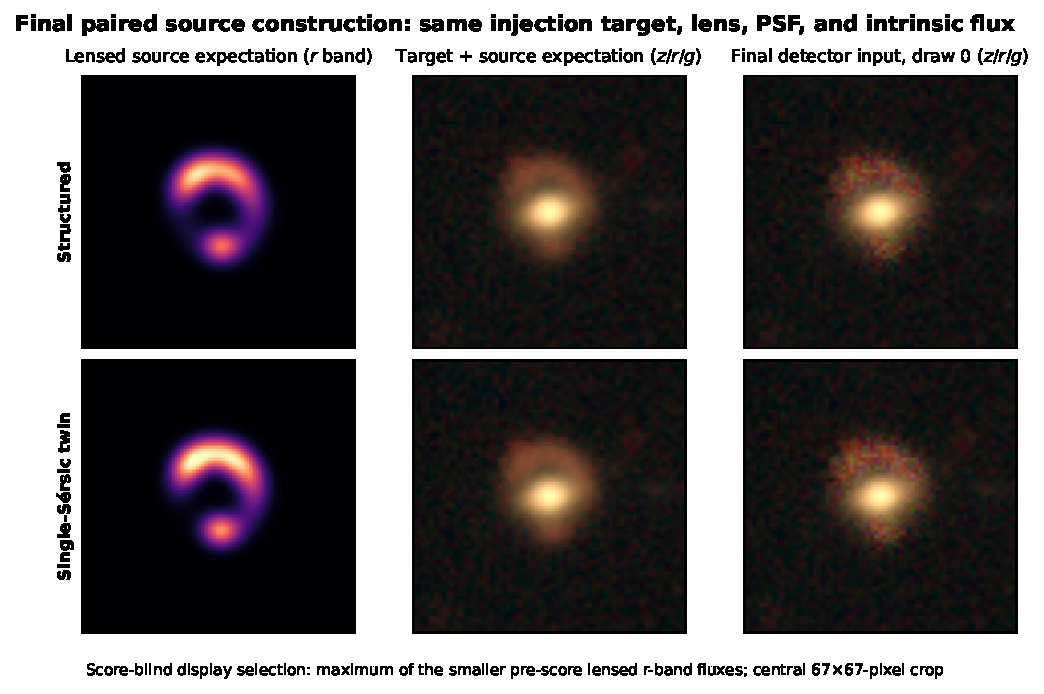
\includegraphics[width=\textwidth]{figures/section3_final_psrc_construction.pdf}
\caption{Illustration from the final \(P_{\rm src}\) bank. The pair is selected
without detector scores by maximizing the smaller of the two pre-score lensed
\(r\)-band fluxes, solely to make the inserted light visible. This display
selection does not alter the analysis population; the pair remains in the
final paired analysis. Rows show the structured
construction and its deterministic single-S\'{e}rsic twin. Columns show the
lensed source expectation in \(r\), the target plus source expectation in
\(z/r/g\) colour, and final photon draw 0 supplied to the detector. The pair
shares the target, source identity, lens mapping, nominal source-plane centre,
effective PSF, intrinsic per-band flux, and photon coupling, but receives no post-lensing
flux rescaling. Panels use the central \(67\times67\)-pixel display crop; the
detector uses all \(101\times101\) pixels.}
\label{fig:final_psrc_construction}
\par\smallskip{\raggedright\noindent\textit{Alt text:} Two rows compare the structured
source and its smooth single-S\'{e}rsic twin. The first column shows similar
but visibly non-identical ring-like \(r\)-band source expectations. The second
shows each expectation added to the same bright central survey galaxy. The
third shows photon draw 0, where coupled source-photon fluctuations are
visible around the shared foreground scene.\par}
\end{figure*}

\subsection{Paired source construction}
\label{sec:paired_source_construction}

The final \(P_{\rm src}\) design has 99 target-cell--radius blocks. Each block
contains 16 distinct targets, with four from each within-cell
intrinsic-\(r\)-magnitude quantile and one assignment from each source
stratum. This gives 1,584 pairs on distinct targets; each of the 144 empirical
sources is used 11 times.

Targets are ordered by a namespaced SHA-256 hash within each cell and
intrinsic-magnitude quantile before four are assigned to each radius. Parent
scenes are then ordered within cell--radius blocks, and the 16 source strata
are cycled deterministically across those blocks using the hash-ordered source
rosters. The assignment uses no detector score, threshold decision, or probe
feature.

Within a pair, the structured and deterministic single-S\'{e}rsic maps share
the exact target, lens and shear parameters, source position,
aligned source-plane centroid, effective per-band PSF, intrinsic \(g/r/z\) fluxes,
renderer, and photon draw indices. The primary design fixes intrinsic flux
before lensing and applies no post-lensing rescaling. Differences in
magnification induced by the two source maps therefore remain part of the
source-construction intervention. The realised flux centroids are not explicitly aligned
after rendering.

A separate design pilot uses disjoint targets and sources under the same
cell, radius, magnitude, and source-stratum structure. Eight is the smallest
tested draw count meeting its paired-risk MCSE criterion; Appendix
Table~\ref{tab:psrc_draw_pilot} gives the candidate panel.

The comparison in Section~\ref{sec:paired_source_estimators} therefore
isolates the two complete source-construction pathways at the same intrinsic
flux and nominal source-plane centre.

\subsection{Renderer validation}
\label{sec:renderer_validation}

A stratified 142-scene audit evaluates quadrature, an independently refined
integration, an effective-PSF reference, and SIE deflections from Lenstronomy
\citep{Birrer2018}. Appendix~\ref{app:renderer_reconciliation} reports its
support and numerical bounds. These tests assess numerical accuracy for the
configurations examined; they do not test whether the adopted source, lens,
PSF, or detector models are astrophysically complete.

\section{Analysis design and statistical methods}
\label{sec:analysis_design}

This section defines the operating points, estimators, and uncertainty
procedures used for the experiment sets in Table~\ref{tab:simulation_sets}.

\subsection{Evaluation cohorts, scoring procedure, and operating points}
\label{sec:scoring_contract}

The primary selected-system endpoint uses the 43-system evaluation cohort
defined in Section~\ref{sec:data_partitions}. None was used for detector
fitting or validation, detector-model selection, threshold calibration, or
exploratory feature-analysis development. The 20 systems assigned to that
exploratory role are excluded from this denominator.

Two disjoint catalogue-negative samples are drawn as whole spatial groups
from the detector's negative test population. The threshold sample contains
20,002 rows in 1,768 spatial groups. A second sample contains 12,512 rows in
1,089 spatial groups and is used only to measure the achieved FPR without
modifying the calibrated threshold.

For the primary analyses, the selected-system endpoint, \(G_{\rm rec}\),
\(P_{\rm noise}\), and \(P_{\rm src}\) use the same epoch-160
EfficientNetV2-S checkpoint, preprocessing, and scoring procedure. The
network is in evaluation mode:
all batch-normalisation layers use stored running statistics and dropout is
inactive. Inference uses float32 operations.
Logits define the operating point because extreme float32 sigmoid values can
saturate numerically. The displayed
\(p=\operatorname{sigmoid}(\ell)\) is not treated as a calibrated
probability. Execution-environment and batching details are reported in
Appendix~\ref{app:technical_validation}.

For \(N_0\) calibration negatives with native float32 logits sorted in
descending order
\(s_{(1)}\geq\cdots\geq s_{(N_0)}\), a target FPR \(\alpha\) permits
\(k=\lfloor\alpha N_0\rfloor\) exceedances. We choose
\begin{equation}
\begin{aligned}
 t_\alpha
 &=\operatorname{nextafter}_{32}\!\left(s_{(k+1)},+\infty\right),\\
 D_i(t_\alpha)&=\mathbb{I}(\ell_i\geq t_\alpha).
\end{aligned}
\label{eq:common_threshold}
\end{equation}
With \(N_0=20\,002\), \(\alpha=10^{-3}\), and \(k=20\),
this gives \(t_{10^{-3}}\simeq1.572\) and 20 calibration exceedances. The
full-precision float32 value is reported in
Appendix~\ref{app:technical_validation}. The threshold is applied unchanged
to every primary detector-response analysis; the feature probes do not use it.

\subsection{Detector-checkpoint sensitivity}
\label{sec:checkpoint_sensitivity_methods}

The primary detector is the seed-42 epoch-160 checkpoint trained with reviewed
and additional catalogue candidates. The sensitivity analysis selects the
highest-validation-AP checkpoint from each of the 12 training runs, retaining the earlier epoch
under ties. Each checkpoint receives its own threshold from the same
calibration sample using Equation~\ref{eq:common_threshold}, and that
threshold is applied to the common evaluation data.
The target \(10^{-3}\) defines the empirical calibration rate.
Checkpoint-specific estimates and intervals condition on \(t_m\).

The pixels, estimators, and dependence-aware resampling procedures are
unchanged across checkpoints; only model weights, scores, and thresholds
vary. The operational \(G_{\rm domain}\) and \(G_{\rm match}\) probes
characterize only the designated primary checkpoint and are not repeated
across the panel. The panel tests how thresholded detector responses change
across trained models; the feature-space analysis is performed only for the
primary detector. The 12 checkpoints are correlated variants within one
detector design \citep{Schaefer2018,Canameras2024}. We report both
validation-selected and terminal-epoch checkpoints; comparisons between
these checkpoint policies are exploratory.

\subsection{Detector-performance and recovery estimators}
\label{sec:performance_estimators}

For a labelled population at a stated threshold, recall is
\({\rm TP}/({\rm TP}+{\rm FN})\), FPR is
\({\rm FP}/({\rm FP}+{\rm TN})\), and precision is
\({\rm TP}/({\rm TP}+{\rm FP})\). ROC AUC measures ranking across all
thresholds, with half credit for ties. The reported precision--recall summary
is average precision. The Brier score is
\begin{equation}
 B = \frac{1}{n}\sum_{i=1}^{n}(p_i-y_i)^2 .
\label{eq:brier_score}
\end{equation}
Validation-positive metrics use noisy reviewed and additional catalogue
candidate labels and are development diagnostics, not estimates on confirmed
systems.

For a named injection population \(Q\), recovery at threshold \(t\) is
\begin{equation}
 \widehat C_Q(t)
 = \frac{1}{|Q|}\sum_{i\in Q}\mathbb{I}(\ell_i\geq t).
\label{eq:conditional_recovery}
\end{equation}
This quantity is conditional on the target population, source and mass-model
priors, observing-condition grid, visibility policy, detector, and threshold
specified for \(Q\). We call this quantity conditional recovery rather than
survey-population completeness.
Because \(G_{\rm rec}\) imposes no independent detectability or visibility
condition, its recovery fraction combines configurations that may not be
physically detectable with the finder's response; it is not an estimate of
finder response conditional on detectability alone.

For \(x\) row-level successes among \(n\) rows, the 95 per cent Wilson score
interval \citep{Wilson1927} is
\begin{equation}
\begin{aligned}
 p_{\rm W} &=
 \frac{\widehat p+z^2/(2n)}{1+z^2/n},\\
 \Delta_{\rm W} &=
 \frac{z}{1+z^2/n}
 \sqrt{\frac{\widehat p(1-\widehat p)}{n}+\frac{z^2}{4n^2}},
 \\
 {\rm CI}_{\rm W} &= [p_{\rm W}-\Delta_{\rm W},p_{\rm W}+\Delta_{\rm W}],\\
 \widehat p &= x/n,\qquad z=\Phi^{-1}(0.975)\simeq1.96 .
\end{aligned}
\label{eq:wilson_interval}
\end{equation}
We apply this row-level interval to the achieved-FPR endpoint. Because nearby
catalogue rows can be dependent, that endpoint also receives a 10,000-draw
spatial-group interval: each draw assigns one independent mean-one
exponential multiplier to each spatial group and takes the weighted ratio of
exceedances to rows. The Wilson and multiplier intervals correspond to
different dependence summaries. The 43 selected confirmed systems are
reported as an exact finite cohort without a binomial or population interval.

For \(G_{\rm rec}\), let \(D_{chr}\) be the threshold indicator for target
\(h\) in retained observing cell \(c\) at radius \(r\). With nine cells, 500
targets in each cell, and 11 radii per target, the primary point estimator is
\begin{equation}
\widehat C_{\rm rec}
=\frac{1}{9}\sum_{c=1}^{9}\frac{1}{500}\sum_{h=1}^{500}
  \frac{1}{11}\sum_{r=1}^{11}D_{chr}.
\label{eq:grec_balanced_recovery}
\end{equation}
Thus cells, targets within cells, and the 11 radius nodes receive equal
weight. This equals the raw row mean because the design is balanced; it is
not a survey-population weighting.

Sampling uncertainty uses 10,000 exponential-multiplier draws at the
injection-target spatial-group level. A group receives one global multiplier
per draw, and that same multiplier follows all of its targets wherever they
occur across cells and follows every radius of each target. Within each cell,
the weighted target mean is formed as a ratio. To remove finite-draw ratio
bias without changing the joint covariance, the draw distribution for every
cell--radius entry is recentered to its exact equal-target point estimate.
The overall 95 per cent interval is the 2.5th and 97.5th percentiles of the
recentered, equal-cell and equal-radius draws.

The radius curve averages cells and targets at each radius. Its unstudentised
simultaneous band uses
\begin{equation}
\begin{aligned}
 q_{0.95}
 &=\operatorname{quantile}_{0.95}
 \left(
 \left\{\max_r\left|\widehat C^{*(b)}_r-\widehat C_r\right|\right\}
 _{b=1}^{10000}\right),\\
 {\cal B}_r&=[\widehat C_r-q_{0.95},\,\widehat C_r+q_{0.95}] .
\end{aligned}
\label{eq:grec_simultaneous_band}
\end{equation}
The band is not clipped to \([0,1]\). Every cell--radius estimate has 500
distinct targets; the resampling unit, rather than the injection count,
defines independent support.

\subsection{Linear probes and grouped evaluation}
\label{sec:linear_probe_methods}

A linear probe consists of fold-local standardisation followed by
\(L_2\)-regularised logistic regression on features computed with encoder
weights held fixed. Every probe uses \(C=1\), the \texttt{lbfgs} solver,
\texttt{max\_iter}=5000, estimator seed 42, and scikit-learn 1.9.1. The
weighted mean and variance used by \texttt{StandardScaler} are fitted only on
the training folds, and the same training weights are supplied to the
logistic-regression fit.

Dependency groups are defined without examining feature values. They are the
transitive union of shared physical group, NSIDE\(=128\) NESTED HEALPix cell
\citep{Gorski2005}, within-population spatial group, reference identity,
injection-target identity and underlying-scene identity, source, lens, PSF, renderer and
render-parameter identities, random-draw identity, and base or final pixel
hash. Every resulting dependency component remains wholly in one of five
folds; score-blind fold allocation uses seed 42. This closes indirect links,
including a reference geographically linked to an injection target in a
different nominal pair.

Across the full set of rows eligible to fit an axis, the two fitting classes
receive equal total base weight. Within a class, every dependency component receives equal total
weight, divided equally over its rows. Each fold fit uses the corresponding
weights of its retained training components without fold-specific
renormalisation. For fitting-roster size \(N\), class \(y\) represented by
\(K_y\) components, and \(n_{c,y}\) class-\(y\) rows in component \(c\), the
weight is
\begin{equation}
 w_i=\frac{N}{2K_y n_{c,y}}.
\label{eq:probe_weights}
\end{equation}
For \(G_{\rm domain}\), the weights sum to 6,379, with 3,189.5 assigned to
each class. Consequently, repeated radii from one connected target do
not receive eleven times the training weight of a singleton component. The
same full-roster component-equal, class-balanced weights define the primary
pooled out-of-fold (OOF) ROC AUC. A row-weighted OOF AUC is retained only as
a diagnostic.
ROC AUC uses half credit for tied positive--negative scores.

The domain probe compares all 43 selected confirmed systems with the exact
6,336-row \(G_{\rm domain}\) subset in 576 injection targets. The common
dependency graph contains 561 components: 43 contain observed rows, 520
contain simulated rows, and two contain both. There are zero component
crossings over the five folds. The comparison uses four feature sets. The
operational representation \(z(x)\) is the 1,280-component output after the
primary detector's global-average-pooling layer and before its dropout and
linear classifier. The existing lens head evaluates
\begin{equation}
 h(x)=w_{\rm lens}^{\mathsf T}z(x)+b .
\label{eq:fixed_head}
\end{equation}
The operational domain probe instead fits fold-specific regularized linear
readouts of fold-standardized \(z(x)\) to observed-versus-injected labels,
using training rows only. This examines the representation that feeds the
finder without restricting the diagnostic to its learned lens-classification
direction. The existing lens head is reported as a fixed-score baseline
alongside the four fitted feature protocols. Both use the
detector-native full \(101\times101\) \(g,r,z\) input with the trained mapping
defined in Section~\ref{sec:preprocessing}.

The Stein representation is the 2,048-component global-average-pooled output
of its self-supervised ResNet-50 before the projection head
\citep{Stein2022}. Its encoder was trained with a contrastive objective on
unlabelled Legacy Survey images. Object-level overlap between those
pretraining images and the present cutouts is unknown, so the Stein result is
interpreted as feature-protocol sensitivity. The generic ImageNet
representation is the 1,280-component global-average-pooled output of a
separate EfficientNetV2-S, with different weights from the lens-label-conditioned
operational detector. The fourth representation contains 18 fixed pixel
statistics. Each representation includes its own preprocessing. The two
external deep encoders use the Legacy Survey display mapping adopted by
\citet{Stein2022}. For nanomaggy
channels \(x_c\), let \(u_c=a_cx_c+m\), with
\((a_g,a_r,a_z)=(6.0,3.4,2.2)\), \(m=0.03\), and \(q=20\). The exact mapping is
\begin{equation}
\begin{aligned}
 I&={1\over3}\sum_{c\in\{g,r,z\}}\max(0,u_c),\\
 F(I)&={\operatorname{asinh}(qI)\over\sqrt q\,I_{\rm safe}},\\
 (R,G,B)&=\operatorname{clip}_{[0,1]}\!\left[(u_z,u_r,u_g)F(I)\right],
\end{aligned}
\label{eq:rgb_preprocessing}
\end{equation}
where \(I_{\rm safe}=I+10^{-6}\mathbf{1}[I=0]\). The Stein input is
the central \(96\times96\) pixels. The ImageNet input uses all
\(101\times101\) pixels, is bilinearly resized with antialiasing to
\(384\times384\), and receives the standard ImageNet channel normalisation.
The pixel representation records, separately in each \(g,r,z\) band, the
mean, standard deviation, median, 99th percentile, minimum, and maximum.
Probe comparisons therefore diagnose the frozen representation together with
its preprocessing, not encoder weights alone.

\(G_{\rm domain}\) reports dependency-component-equal pooled OOF AUCs as
finite-cohort, model-conditional point estimates. No resampling interval or
significance test is attached. We compare all four representations on the
same rows, folds, component weights, and observed--injected labels. The five
fold-level AUCs show how performance varies across held-out subsets containing
only eight or nine observed systems.

\subsection{Unpaired separation and matched controls}
\label{sec:decomposition_methods}

We distinguish three questions. An unpaired real--injection probe asks whether
the selected populations are separable. A real--bare-target probe measures
separation present before an arc is added. A bare--injected comparison holds
the target fixed and measures how the added arc moves that target in feature
space. We interpret these estimands separately because they answer different
population and paired-movement questions.

The matched-baseline set \(G_{\rm match}\) uses the exact 43 selected confirmed
systems as observed references. They are matched without replacement to the
4,500 \(G_{\rm rec}\) injection targets on observed \(z\)-band magnitude,
catalogue S\'{e}rsic index, axis ratio, \(r\)-band PSF FWHM, and \(r\)-band
depth. No detector score or representation feature enters matching.

For each covariate \(k\), the complete 4,500-target sample supplies the median
\(m_k\) and interquartile range \(s_k\), using all finite values of that
component. We define \(z_{ik}=(x_{ik}-m_k)/s_k\). All five values must be
finite for a target to be eligible; all 4,500 targets meet this requirement,
and no imputation is used. A reference--target edge is allowed only when
\begin{equation}
\begin{aligned}
 |z_{{\rm ref},k}-z_{{\rm target},k}|&\leq2
 &&\text{for every }k,\\
 \left[\sum_k(z_{{\rm ref},k}-z_{{\rm target},k})^2\right]^{1/2}
 &\leq3 .
\end{aligned}
\label{eq:gmatch_calipers}
\end{equation}
Among allowed edges, maximum-cardinality then minimum-total-distance
assignment is used, with SHA-256-sorted identifiers breaking ties. All 43
references are matched to unique targets.

The supplementary material includes the complete full-field reference--target
atlas, the matching and brightness-parent tables, covariate balance summaries,
and the code used to generate the displays.

Each target contributes its exact stored bare cutout and its exact
\(\theta_{\rm E}=1.5\)-arcsec \(G_{\rm rec}\) deterministic expectation image. There is no
rerendering, post-render selection, flux rescaling, imputation, replacement,
or target-brightness floor. The resulting 43 observed--bare--injected
triplets form 43 closed dependency components.

In each representation and fold, the logistic axis is fitted only to the
training-fold observed and bare rows, with observed as the positive direction;
injected rows fit neither the axis nor its scale. Let \(a_{jf}^{x}\) denote a
held-out decision-function score for target \(j\), fold \(f\), and arm
\(x\in\{{\rm bare},{\rm inj}\}\). We standardise both arms using the weighted
mean \(\mu_f^{\rm bare}\) and population standard deviation
\(\sigma_f^{\rm bare}\) of the training-fold bare scores:
\begin{equation}
\begin{aligned}
\widetilde a_{jf}^{\,x}
&=\frac{a_{jf}^{x}-\mu_f^{\rm bare}}{\sigma_f^{\rm bare}},\\
M_j&=\widetilde a_{jf}^{\,{\rm inj}}-\widetilde a_{jf}^{\,{\rm bare}},
\qquad
\widehat\Delta_{\rm match}=\frac{1}{43}\sum_{j=1}^{43}M_j .
\end{aligned}
\label{eq:gmatch_movement}
\end{equation}
Here \(M_j\) is an equal-target movement measured in training-bare
standard-deviation units toward the observed-reference side of a cross-fitted
axis.

Pooled observed--bare, observed--injected, and injected--bare AUCs, with half
credit for ties, summarize the same fitted axis. These point summaries
condition on the frozen score-blind assignment; no formal interval or
significance test is attached. The matching set contains five measured
central-object and observing quantities; complete photometric-redshift and
source-magnitude covariates are unavailable, and the observed central-object
quantities can include lensed-source light.

\subsection{Fixed-target brightness and source-photon response}
\label{sec:bounded_control_methods}

\(C_{\rm bright}\) uses equation~\eqref{eq:brightness_control} on 43 fixed
targets under the detector's trained 20--32-pixel annulus and clip-10
preprocessing. For each target and magnitude, photon indicators are first
averaged over the eight keyed draws; the resulting target-level values are
then averaged equally over targets. Primary summaries are recovery and
native-logit response over magnitude; photon-minus-expectation is the paired
secondary contrast. If \(\widehat R_d\) is the equal-target photon recovery at
one magnitude for draw index \(d\), the finite-draw diagnostic is
\begin{equation}
 {\rm MCSE}_{\rm bright}
 =\frac{{\rm sd}(\widehat R_1,\ldots,\widehat R_8)}{\sqrt{8}} .
\label{eq:brightness_mcse}
\end{equation}
No population interval or visibility admission rule is attached. Source-only
in-stamp flux and peak intensity are diagnostics rather than calibrated arc
S/N.

\subsection{Arc-level Poisson experiment}
\label{sec:poisson_methods}

\(P_{\rm noise}\) compares all 49,500 stored \(G_{\rm rec}\) expectations
with eight modelled source-photon realizations per scene at
\(g=150\ {\rm e^{-}\,nmgy^{-1}}\), using the common threshold. The target
and expected arc remain fixed; only source-photon realization changes
(Section~\ref{sec:noise_model}).

Let \(D^{\rm E}_{chr}\) denote the deterministic expectation decision and
\(D^{\rm M}_{chrd}\) the modelled-photon decision for draw \(d\). The primary
modelled-photon-minus-expectation estimand is
\begin{equation}
\widehat\Delta_{\rm noise}
=\frac{1}{9}\sum_{c=1}^{9}\frac{1}{500}\sum_{h=1}^{500}
 \frac{1}{11}\sum_{r=1}^{11}
 \left\{\frac{1}{8}\sum_{d=1}^{8}D^{\rm M}_{chrd}-D^{\rm E}_{chr}\right\}.
\label{eq:pnoise_risk_difference}
\end{equation}
Photon draws are therefore averaged within deterministic expectation scene
before radii are averaged within target; targets and retained cells then
receive equal weight. Repeated photon draws never increase a target's
scientific weight.

The sampling interval uses 10,000 target-spatial-group exponential-multiplier
draws with the same global grouping, equal-cell weighting, and cell--radius
recentering as \(G_{\rm rec}\). Its uncertainty is conditional on the
realized target and source construction and does not include gain-model or
threshold-calibration uncertainty. The radius-specific effects receive the
same maximum-absolute-deviation simultaneous-band construction as
equation~\eqref{eq:grec_simultaneous_band}. Gained and lost threshold
crossings are reported as descriptive probabilities over the complete
scene--draw rows.

For scene \(i\), let \(s_i^2\) be the sample variance of its eight modelled
threshold indicators and let \(w_i=1/49\,500\), which is the final
equal-cell, equal-target, equal-radius weight under the balanced design. The
finite-draw contribution is
\begin{equation}
 {\rm MCSE}_{\rm noise}
 =\left(\sum_{i=1}^{49\,500}w_i^2\frac{s_i^2}{8}\right)^{1/2}.
\label{eq:pnoise_mcse}
\end{equation}
The estimate applies to the specified stochastic source-photon model, whose
\(g=150\) conversion and post-coadd construction define the intervention.

\subsection{Paired source estimators}
\label{sec:paired_source_estimators}

For pair \(j\) and photon draw \(d\), let \(D^{\rm ser}_{jd}\) and
\(D^{\rm str}_{jd}\) indicate whether the corresponding photon-realized images
from the single-S\'{e}rsic and structured constructions exceed the common
logit threshold. The underlying source constructions are deterministic, but
the scored rows are draw-specific images. The primary estimand is the
S\'{e}rsic-minus-structured photon-averaged risk difference,
\begin{equation}
\widehat\Delta_{\rm src}
=\frac{1}{1584}\sum_{j=1}^{1584}\frac{1}{8}\sum_{d=1}^{8}
 \left(D^{\rm ser}_{jd}-D^{\rm str}_{jd}\right).
\label{eq:psrc_risk_difference}
\end{equation}
Operationally, draw differences are first averaged within pair; pairs are
then averaged within each of the nine fixed target cells and cells are
averaged equally. The expression above is identical because every cell has
the same number of pairs, every cell--radius block contains all 16 source
strata, every selected source is used 11 times, and all base analysis weights
are one.

The 95 per cent interval is a 10,000-draw multiway exponential-multiplier
interval. Each draw assigns one global mean-one exponential multiplier to
each of the 1,219 target spatial groups and applies it to that group's rows in
every cell and radius. It independently assigns one multiplier to each of the
144 empirical sources; source multipliers are normalised to mean one within
each of the 16 fixed source strata. The product of the spatial and source
multipliers weights each pair, after which equal-cell ratio estimates are
averaged. Draws are recentered to \(\widehat\Delta_{\rm src}\), and the 2.5th
and 97.5th percentiles form the reported interval. This procedure preserves
dependence from repeated sources and geographically linked targets. The
resulting interval is a design-based approximation, not an exact
binary-outcome interval.

Finite-photon-draw Monte Carlo uncertainty is reported separately. Let
\(\widehat\Delta_d\) be the same equal-cell risk difference computed from
draw index \(d\) alone. Then
\begin{equation}
 {\rm MCSE}_{\rm src}
 =\frac{{\rm sd}(\widehat\Delta_1,\ldots,\widehat\Delta_8)}{\sqrt{8}} .
\label{eq:psrc_mcse}
\end{equation}
The point estimate and multiplier interval condition on the
calibrated threshold. The empirical construction retains measurement
uncertainty, making the estimand a comparison of the complete
source-construction pathways.

\subsection{Interpretation of estimates and intervals}
\label{sec:reporting_methods}

The achieved-FPR, \(G_{\rm rec}\), \(P_{\rm noise}\), and \(P_{\rm src}\)
intervals use the 95 per cent procedures defined above. The selected
43-system endpoint and both feature-probe analyses are finite-cohort point
summaries without population intervals. The four feature protocols form one
finite-cohort comparison. The operational probes characterize the primary epoch-160
checkpoint; the 12-checkpoint panel evaluates thresholded detector-response
sensitivity and does not repeat the feature probes.

Each thresholded estimate conditions on the threshold calibrated
for its checkpoint.
Multiplier intervals describe the specified target/source dependence but do
not incorporate detector-training, threshold-calibration, gain-model, source
reconstruction, or population-transport uncertainty. Finite-photon MCSE is
reported separately from sampling uncertainty. Formal equivalence assessment
would require a predefined margin beyond these estimation summaries.

\section{Results}
\label{sec:results}

\subsection{Validation context and disjoint endpoints}
\label{sec:current_detector_results}

The operating threshold was calibrated on 20,002 catalogue-negative examples
before endpoint scoring. At \(t_{10^{-3}}=1.572\), 20 calibration examples
met or exceeded threshold; Appendix~\ref{app:technical_validation} gives the
full-precision float32 value and comparison rule.

In the separate achieved-FPR endpoint, 13 of 12,512 catalogue-negative rows
exceed \(t_{10^{-3}}\), or 0.104 per cent. The row-Wilson 95 per cent
interval is [0.061, 0.178] per cent, and the spatial-group multiplier
interval is [0.055, 0.166] per cent. This is the threshold-exceedance rate for
the fixed evaluation cohort at the previously calibrated operating point.

The detector also responds to 39 of the 43 selected confirmed systems
(90.7 per cent). We report this selected-cohort fraction without a population
interval because the systems combine heterogeneous discovery programmes,
catalogue eligibility, and galaxy- and cluster-scale lenses.
Section~\ref{sec:checkpoint_sensitivity_results} reports this endpoint for the
12 sensitivity checkpoints. Appendix~\ref{app:technical_validation} reports
the separate noisy-label development diagnostics; threshold calibration and
selected-system evaluation use the cohorts defined above.

\subsection{\(G_{\rm domain}\) linear-probe separation}
\label{sec:domain_probe_results}

Observed references and simulated injections are distinguishable in all four
feature protocols (Table~\ref{tab:gdomain_four_rep}). Cross-fitted
domain-ranking AUC is 0.991 in the
operational detector's pooled penultimate representation, 0.958 in Stein
self-supervised survey features, 0.979 in generic ImageNet features, and
0.981 in pixel statistics. Thus strong separation appears in the lens-trained
representation, external learned representations, and elementary image
summaries.

\begin{table*}
\caption{Domain-ranking AUC on the same 43 observed and 6,336 injected rows.
The first four rows are cross-fitted domain probes. ``Fold range'' gives their
minimum and maximum fold AUC; folds contain only 8 or 9 observed systems. The
fixed operational lens head is a non-cross-fitted baseline on the same roster
and weights.}
\label{tab:gdomain_four_rep}
\centering
\begin{tabular}{lrrrl}
\toprule
Readout & Dimension & Domain-ranking AUC & Fold range & Evaluation \\
\midrule
Operational penultimate & 1\,280 & 0.991340 & 0.985--0.999 &
Cross-fitted domain probe \\
Stein SSL & 2\,048 & 0.958187 & 0.929--1.000 &
Cross-fitted domain probe \\
Generic ImageNet & 1\,280 & 0.978528 & 0.953--0.994 &
Cross-fitted domain probe \\
Pixel statistics & 18 & 0.980745 & 0.938--0.997 &
Cross-fitted domain probe \\
\midrule
Fixed operational lens head & -- & 0.980306 & -- &
Not cross-fitted \\
\bottomrule
\end{tabular}
\end{table*}

The existing lens-classification head also separates these populations
strongly (Table~\ref{tab:gdomain_four_rep}), showing that the difference is
expressed in the operational score as well as the fitted penultimate readouts.
The two readouts share a feature vector; no significance test compares their
AUCs. Each finite-cohort AUC describes its feature protocol, including its
training history, preprocessing, and fitted readout. Native-score summaries appear in
Appendix~\ref{app:four_representation_diagnostics}.

\subsection{\(G_{\rm match}\) shared-axis diagnostics}
\label{sec:matched_probe_results}

The score-blind \(G_{\rm match}\) design contains 43 triplets: each selected
observed reference, one matched bare \(G_{\rm rec}\) target, and that target with
its fixed 1.5-arcsec injection. The cross-fitted axis in each representation
is learned from observed-reference and bare-target rows only; injected rows are
not used to fit the axis or its scale. There are 129 rows in 43 dependency
components. Appendix Table~\ref{tab:gmatch_coverage} reports the measured
reference, complete-target-roster, and matched-target covariate ranges.

Mean injected-minus-bare movement along the operational observed--bare axis is
\(+0.023\), with median \(+0.0175\), in training-bare standardized-score
units. Twenty-seven targets move toward the observed-positive side and 16 in the
opposite direction; individual movements range from \(-0.453\) to \(+0.998\).
The mean signed movement is therefore near zero despite heterogeneous
pairwise shifts. The pooled injected-versus-bare AUC on this axis is 0.509.
Unlike \(G_{\rm domain}\), this analysis asks how adding a fixed source moves
the same target along an axis fitted between observed systems and bare
targets. Mean movements in Stein,
ImageNet, and pixel features are \(+0.235\), \(+0.025\), and \(-0.029\),
respectively. The Stein movement distribution is asymmetric: its median is
\(-0.069\), 12 movements are positive and 31 negative, and the range is
\(-0.982\) to \(+5.204\). It therefore does not indicate that most matched
targets move toward the observed side. Table~\ref{tab:gmatch_final} reports
the corresponding pooled AUCs.

Among 18 statistics, the \(z\)-band median has univariate AUC 0.888, and
omitting it lowers multivariate pixel AUC from 0.981 to 0.932 in
\(G_{\rm domain}\). Separately, within the 43 \(G_{\rm match}\) triplets, its
unweighted finite-cohort mean is 0.011448 in observed references, 0.005088 in
bare targets, and 0.005094 after injection. This matched bare--injected
comparison shows that the leading observed--injected offset is already present
before source insertion. This pixel-level result does not establish which
features drive the operational detector.

\begin{table*}
\caption{\(G_{\rm match}\) shared-axis pooled OOF AUC diagnostics for the 43
triplets. The axis is fitted on observed and bare rows; all entries are
finite-cohort point estimates without formal intervals.}
\label{tab:gmatch_final}
\centering
\small
\setlength{\tabcolsep}{4pt}
\begin{tabular}{lrrr}
\toprule
Representation & Obs.--bare & Obs.--inj. & Inj.--bare \\
\midrule
Operational penultimate & 0.998 & 0.998 & 0.509 \\
Stein SSL & 0.979 & 0.982 & 0.488 \\
ImageNet & 0.973 & 0.971 & 0.500 \\
Pixel statistics & 0.928 & 0.933 & 0.478 \\
\bottomrule
\end{tabular}
\end{table*}

\subsection{Conditional recovery and fixed-target brightness response}
\label{sec:recovery_results}

Conditional \(G_{\rm rec}\) recovery is 3.45 per cent (95 per cent
spatial-group interval, 3.10--3.83 per cent) under equal weighting of
observing cells, injection targets, and Einstein radii. This is 1,710
detections among 49,500 scenes generated from 4,500 targets in 2,187 spatial
groups. Two bare
targets exceed the same threshold. Across target--radius comparisons, 22 are
positive both before and after injection, 1,688 become positive, none becomes
negative, and 47,790 remain negative. The injection therefore raises the
positive-call rate by 3.41 percentage points across the specified grid.

The grid applies no rendered-arc visibility or S/N admission rule; its
estimand therefore averages all designed scenes rather than a visibility-selected
subset. Scene-weighted recovery is 8.45, 1.90, and 0.12 per cent in intrinsic source-magnitude bins
\([23,24)\), \([24,25)\), and \([25,26)\), respectively
(Table~\ref{tab:grec_brightness}). The final design also contains 99
cell--radius estimates: 500 targets at each radius in each of nine occupied
PSF--depth cells. Appendix~\ref{app:cell_radius_response} reports that
conditional response surface and its one empty PSF--depth combination.

Figure~\ref{fig:grouped_recovery} shows the equal-cell, equal-target response by
Einstein radius. Recovery is 0.044 per cent at 0.5 arcsec, reaches 6.22 per
cent at 2.5 arcsec, and is 6.02 and 5.47 per cent at 2.75 and 3.0 arcsec.
The simultaneous 95 per cent band has half-width 0.82 percentage points.

\medskip
\begin{center}
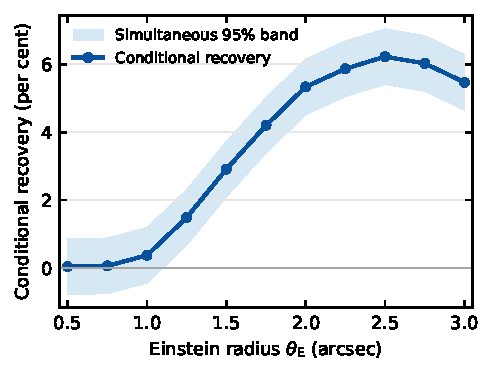
\includegraphics[width=\columnwidth]{figures/section5_grouped_recovery.pdf}
\end{center}
\refstepcounter{figure}\label{fig:grouped_recovery}
\noindent\textbf{Figure~\thefigure.} Conditional \(G_{\rm rec}\) recovery at the
\(t_{10^{-3}}\) threshold versus Einstein radius. Points are equal-cell,
equal-target estimates; shading is the simultaneous 95 per cent
target-spatial-group multiplier band. The ordinate is conditional recovery over
the designed scenes.
\par\smallskip\noindent\textit{Alt text:} A line rises from near-zero recovery
at 0.5 arcsec to about 6.2 per cent at 2.5 arcsec, then declines modestly.
A shaded simultaneous interval surrounds the line.
\medskip

In the separate \(C_{\rm bright}\) fixed-target experiment,
expectation-image recovery is 6/43 and 7/43 at intrinsic magnitudes 18.5 and 19.5,
peaks at 8/43 at magnitude 20.5, and then decreases to zero at magnitudes 24.5
and 25.5. Across all eight magnitudes, expectation-image recovery is
non-monotonic; its peak at magnitude 20.5 exceeds each of the two brighter
nodes by two and one targets, respectively.
Photon-minus-expectation estimates range from \(-3.20\) to \(+2.33\)
percentage points through magnitude 23.5, with finite-draw MCSE at most 1.07
points. These are responses of the same 43 targets with one retained source
configuration per target and characterize detector response to source scaling
over the tested magnitude range.

\subsection{\(P_{\rm noise}\) photon intervention}
\label{sec:poisson_results}

After equal weighting of cells, targets, and radii, modelled source-photon
noise reduces recovery by 1.20 percentage points (95 per cent
target-spatial-group interval, \(-1.39\) to \(-1.03\); MCSE, 0.014). Recovery
declines from 3.45 per cent for expectation images to 2.25 per cent across
photon draws.

By Einstein radius, the simultaneous band includes zero from 0.5 through
1.5 arcsec and lies below zero from 1.75 through 3.0 arcsec. The interval is
conditional on the modelled source-photon law and frozen threshold; it
excludes gain-model and threshold-calibration uncertainty. In particular,
\(g=150\ {\rm e^{-}\,nmgy^{-1}}\) is the adopted approximate effective
conversion for the source-photon intervention.
Appendix~\ref{app:photon_followup} reports the source-photon normalization
replay, finite-gain diagnostic, and Monte Carlo errors.

\subsection{\(P_{\rm src}\) source-construction result}
\label{sec:paired_source_results}

The \(P_{\rm src}\) design contains 1,584 target--source pairs and eight
photon draws per pair. Across the resulting 12,672 pair--draw rows per arm,
the regularized GalSim-deconvolved structured F814W construction produces 220
detections (1.74 per cent), while its deterministic single-S\'{e}rsic twin
produces 291 (2.30 per cent). At draw level, 83 discordant outcomes favour
the S\'{e}rsic arm and 12 favour the structured arm.

The photon-averaged paired difference is \(+0.56\) percentage points in
favour of the single-S\'{e}rsic arm (95 per cent multiway target-and-source
interval, \(+0.28\) to \(+0.93\); MCSE, 0.042). Within this
fixed-intrinsic-flux construction, the result supports higher recovery for the
single-S\'{e}rsic arm. The estimand compares the complete source-construction
pipelines. Despite equal intrinsic band fluxes, the
S\'{e}rsic arm has greater source-only lensed in-stamp \(r\)-band flux in
1,249 of 1,584 pairs and a greater source-only \(r\)-band peak in 1,516 pairs;
the median S\'{e}rsic-to-structured ratios are 1.0417 and 1.1044,
respectively. The higher lensed flux and peak intensity may contribute to the
recovery difference, but the experiment does not isolate their individual
effects. Deleting any one source or target spatial group does not reverse the
sign of the result.

\subsection{Detector-checkpoint sensitivity}
\label{sec:checkpoint_sensitivity_results}

The validation-selected checkpoints span all 12 training runs defined in
Section~\ref{sec:checkpoint_panel_design}. Every model-specific threshold
yields exactly 20 exceedances among the same 20,002 calibration negatives.
The checkpoint panel covers only thresholded detector responses; the
feature-space results use the primary epoch-160 model.
Achieved-FPR counts range from 9 to 21 among 12,512 evaluation negatives; 11
of the 12 spatial-group intervals contain 0.1 per cent. Selected-cohort
response ranges from 35/43 to 39/43, and conditional \(G_{\rm rec}\) from
1.28 to 3.15 per cent.

Across the validation-selected checkpoints, \(P_{\rm noise}\) ranges from
\(-1.16\) to \(-0.51\) percentage points, with all 12 intervals below zero.
Every \(P_{\rm src}\) estimate is positive, from \(+0.07\) to \(+0.43\)
points, but only 7/12 threshold-conditional intervals exclude zero. Under the
terminal-epoch policy all point-estimate directions are retained, all 12
\(P_{\rm noise}\) intervals remain below zero, and 8/12 \(P_{\rm src}\)
intervals exclude zero. The directions are therefore consistent across the
examined policies, while source-effect interval exclusion is policy-dependent.
These are correlated variants of one training programme;
Appendix~\ref{app:checkpoint_sensitivity} reports the full results and
exploratory-policy qualification.

\subsection{Renderer qualification}
\label{sec:renderer_results}

Across 142 realized scenes, production and reference renders agree within the
reported numerical tolerances. The largest relative \(L_1\) difference is
0.0077, the largest centroid difference 0.023 pixels, and the minimum pixel
correlation 0.9999.

No \(G_{\rm rec}\) or \(P_{\rm src}\) scene uses the renderer's softened
near-circular branch. Production-support SIE tests pass; the separate
boundary-specific test does not meet its predefined criterion.

\section{Discussion}
\label{sec:discussion}

The operational detector's penultimate features strongly distinguish the
selected observed and injected populations, showing that its trained
representation can serve as a detector-specific diagnostic. The same
separation appears in self-supervised survey features, generic ImageNet
features, and elementary pixel statistics, so it is not confined to the
lens-trained representation.

The controls add two distinct observations: a leading pixel-statistic offset
predates insertion, and matched injections have a near-zero mean signed
movement along the separately fitted operational observed--bare axis, with
heterogeneous pairwise shifts. The separate recovery, source-photon,
source-construction, and fixed-target brightness experiments characterize
responses to controlled image changes. The matched controls locate differences
that predate injection, while the recovery experiments measure how the fixed
detector responds when source photons, source construction, or brightness are
changed.

\subsection{What the recovery measurements represent}
\label{sec:discussion_recovery}

The detector responds to 39/43 selected confirmed systems but to 3.45 per cent
of the fixed injection grid. These summaries describe different cohorts and
weighting schemes. The selected systems come from heterogeneous discovery
programmes, whereas \(G_{\rm rec}\) averages equally over nine observing
cells, 4,500 targets, and 11 Einstein radii
\citep{Huang2020,Huang2021,Stein2022,Storfer2024,Sonnenfeld2023,Sonnenfeld2024}.

On the 43 fixed targets, expectation-image recovery peaks at magnitude 20.5
and is lower at the two brighter nodes. Thus recovery is non-monotonic over
the tested intrinsic-magnitude range.

\subsection{Feature diagnostics, matching, and mass-model scope}
\label{sec:discussion_deflector}

The fixed lens head is one affine projection of the operational feature
vector. Its AUC of 0.980 shows that the existing score already expresses a
strong separating direction. Using the same cross-fitted readout for all four
representations shows whether the operational features are uniquely sensitive
to population identity. The probe and fixed head are complementary readouts
of the same feature vector, while the pixel-statistic AUC of 0.981 shows that
elementary image summaries also carry a strong separating direction.

The leading native-pixel offset is already present between the observed
references and bare targets (Section~\ref{sec:matched_probe_results}).
Foreground light, background estimation, survey processing, and sample
selection are all plausible contributors to that offset. The measured offset
is present before insertion; these analyses do not separate the possible
contributions listed above.

\(G_{\rm match}\) asks how one fixed injection moves each matched target along
an observed--bare axis. Its operational mean is near zero, but individual
shifts range from \(-0.453\) to \(+0.998\).
The near-zero cohort mean therefore coexists with substantial individual
movements. Matching reduces differences in the five recorded central-object
and observing quantities. The observed--bare readout describes differences
between complete cutouts; insertion measures movement along that readout on
the same targets. Redshift, velocity dispersion, stellar mass, source
properties, and environment remain outside that matching set. The radius
curve similarly describes response over assigned grid values rather than
target-specific inferred lens models.

\subsection{Arc-photon-noise treatment}
\label{sec:discussion_noise}

The negative aggregate photon effect persists across the 12
validation-selected checkpoints
(Section~\ref{sec:checkpoint_sensitivity_results}). The primary checkpoint's
radius-specific band is a different summary: it includes zero through
1.5 arcsec and lies below zero at larger tested radii
(Section~\ref{sec:poisson_results}).

Only the extra shot-noise term associated with injected flux is changed.
The observed target already contains its realised sky, detector, coaddition,
neighbours, and foreground light. The adopted effective gain is approximate,
and the intervention operates on post-coadd cutouts rather than reconstructing
exposure-level correlated noise or resampling. Eight draws control
finite-photon Monte Carlo error for the adopted
\(g=150\ {\rm e^{-}\,nmgy^{-1}}\) source-photon law. Gain-model and
threshold-calibration uncertainty remain outside the reported interval.

\subsection{Source-construction result}
\label{sec:discussion_source}

Under the tested construction, single-S\'{e}rsic recovery is about
0.56 percentage points higher than structured-source recovery. All 12
validation-selected checkpoint estimates have the same sign with
7/12 intervals excluding zero. Under the terminal-epoch policy all 12 estimates
retain that sign, while 8/12 intervals exclude zero. The direction is
therefore consistent across the examined policies, but interval exclusion is
checkpoint-policy-dependent. The estimand compares the two complete
source-construction pipelines.

The empirical arm is constructed from selected high-S/N F814W images by
deconvolution and reconvolution to a common resolution, followed by
non-negative projection, centring, support restriction, and normalization.
Its spatial map therefore contains both source structure and the effects of
measurement and regularization. Each arm reuses its own F814W-derived map
across \(g,r,z\); the tested construction has no colour gradients or
chromatic morphology.
Both arms share the selected targets, assigned SIE-plus-shear mappings,
effective PSF, modelled photon law, threshold, and post-coadd insertion.
In the noiseless known-source test, global flux, centring, and normalization
errors remain within the stated tolerances
(Appendix~\ref{app:source_transfer_followup}).

Future paired studies can vary source support, regularization, correlated
measurement noise, and
band-dependent morphology while continuing to hold targets, lens mappings,
fluxes, and photon draws fixed.

\subsection{Renderer qualification and numerical scope}
\label{sec:discussion_renderer}

Agreement in the fixed 142-scene validation cohort supports the numerical
implementation within its tested configurations
(Appendix~\ref{app:renderer_reconciliation}). These numerical checks do not
test the astrophysical adequacy of the adopted source, lens, PSF, or detector
models.

\subsection{Relation to published pipelines and resolution}
\label{sec:discussion_literature}

Published pipelines differ in their source constructions, deflector
information, and observing regimes: fully simulated \textit{Euclid}-like
images expose selection dependence on source and lens parameters
\citep{Herle2024}, whereas HSC and other recent pipelines use real galaxy
stamps and, in some cases, more tightly constrained deflector information
\citep{Canameras2021,Rojas2022,Schuldt2023,Canameras2024}. These approaches
vary choices beyond the paired structured--S\'{e}rsic intervention studied
here.

Resolution is especially important. At DR10 resolution, the effective PSF
smooths the rendered lensed images and reduces the observable fine structure
inherited from the source templates. HST, \textit{Euclid}, and seeing-limited
ground-based data resolve different source structure, so the magnitude and
direction of source-construction effects can vary with resolution. Source,
mass, PSF, detector, and processing choices should therefore be tested at the
resolution at which a selection function will be applied.

\subsection{Limitations and future work}
\label{sec:limitations}

Inference is restricted to the sampled systems and tested pipelines.
Generalizing these results to another lens population is limited by missing
physical covariates, mass parameters assigned independently of the target
galaxies, single-band source morphology, post-coadd insertion, approximate PSF
and gain models, and unknown overlap with Stein's pretraining data. The
operational evaluations retain the detector's trained 20--32-pixel annulus and
clip-10 map, making that mapping part of the operational estimand.

The detector panel contains 12 correlated variants of one architecture and
training pipeline. Sampler and schedule changes are
evaluated only at seed 42, the positive-example-set contrast changes several
properties together, and no between-checkpoint contrast interval is attached.
Each estimate conditions on an empirically calibrated threshold, so the panel
combines training variation with calibration-tail variation. It therefore
tests variation within this training family rather than across independent
detector architectures.
The operational feature analysis uses only the primary checkpoint. All four
probes share the 43 observed references; dependency-closed folds keep linked
images together, and component-equal weights prevent repeated injections from
receiving disproportionate weight.

Future work should first construct a deflector sample with reliable redshifts,
velocity dispersions or other mass proxies, then assign mass and environment
jointly with observed light. Controlled mass-model factors should include
density slope, composite baryonic and dark components, external convergence,
multiple deflectors, and line-of-sight structure. Each factor should be varied
within matched targets rather than inferred from an unpaired population
contrast.

Source tests should use multiple real-galaxy catalogues and latent-source
methods, band-dependent morphology and colour gradients, with support,
regularization, and correlated noise varied explicitly. The
structured--S\'{e}rsic intervention should be repeated at space-based and
ground-based resolution under the same underlying systems.
Exposure-level injection before coaddition would test PSF, noise correlation,
deblending, masking, and processing provenance that cutout-level addition
leaves fixed.

Future studies should predefine the simulated population, detector, and
thresholds; preserve system- or target-level grouping; report support in every
conditional cell; and combine unpaired comparisons with bare-target and paired
controls. Repeating the diagnostic under such controlled pipeline changes can
identify which changes alter observed--injected separation. Pairing those
changes with selection-function and downstream population-inference metrics
would connect the diagnostic to survey performance.

\section{Conclusions}
\label{sec:conclusions}

We demonstrated a representation-level diagnostic of observed--injected
differences in selected DESI Legacy Imaging Surveys DR10 images. Linear probes
reuse frozen trained features to evaluate this separation directly.
Strong held-out discrimination in the operational finder's penultimate
representation is accompanied by discrimination in survey self-supervised
features, generic ImageNet features, and elementary pixel statistics under the
common dependency-aware procedure. The separation appears in the operational
detector, two external learned representations, and simple pixel statistics.

A leading pixel-statistic offset largely predates insertion, and the
separately fitted operational observed--bare axis has a near-zero mean signed
movement with heterogeneous individual shifts.

Separately, the finder recovers 3.45 per cent of the full grid without a
visibility cut.
Modelled source-photon sampling lowers this response, and the tested paired
single-S\'{e}rsic construction has higher recovery than its regularized
structured counterpart. The brightness control shows how the same targets
respond to source scaling, while the checkpoint panel shows which intervention
results persist across trained models. The combined results show why future
injection pipelines should be compared on matched foreground populations and
observing conditions, with bare-target controls used to separate pre-existing
image differences from the effects of source insertion.

\section*{Acknowledgements}

Author contributions: Aditrivaishnavi Balaji conceived and led the project,
formulated the research questions, designed the study, developed and validated
the software and injection--recovery pipeline, curated the data and verified
its provenance, designed and executed the experiments and statistical
analyses, interpreted the results, produced the figures, tables, and
reproducibility materials, and drafted and revised the manuscript. Parker
T. Johnson supervised and mentored the project, advised on the astrophysical
context, methodology, and scientific interpretation, and critically reviewed
the manuscript. Both authors reviewed and approved the final manuscript.

The Legacy Surveys consist of three individual and complementary projects:
the Dark Energy Camera Legacy Survey (DECaLS; Proposal ID 2014B-0404; PIs:
David Schlegel and Arjun Dey), the Beijing--Arizona Sky Survey (BASS; NOAO
Proposal ID 2015A-0801; PIs: Zhou Xu and Xiaohui Fan), and the Mayall
\(z\)-band Legacy Survey (MzLS; Proposal ID 2016A-0453; PI: Arjun Dey).
DECaLS, BASS, and MzLS together include data obtained, respectively, at the
Blanco telescope, Cerro Tololo Inter-American Observatory, NSF's NOIRLab; the
Bok telescope, Steward Observatory, University of Arizona; and the Mayall
telescope, Kitt Peak National Observatory, NOIRLab. Pipeline processing and
analyses of the data were supported by NOIRLab and the Lawrence Berkeley
National Laboratory (LBNL). The Legacy Surveys project is honoured to be
permitted to conduct astronomical research on Iolkam Du'ag (Kitt Peak), a
mountain with particular significance to the Tohono O'odham Nation.

NOIRLab is operated by the Association of Universities for Research in
Astronomy under a cooperative agreement with the National Science Foundation.
LBNL is managed by the Regents of the University of California under contract
to the U.S. Department of Energy.

This project used data obtained with the Dark Energy Camera (DECam), which was
constructed by the Dark Energy Survey (DES) collaboration. Funding for the DES
Projects has been provided by the U.S. Department of Energy, the U.S. National
Science Foundation, the Ministry of Science and Education of Spain, the
Science and Technology Facilities Council of the United Kingdom, the Higher
Education Funding Council for England, the National Center for Supercomputing
Applications at the University of Illinois at Urbana--Champaign, the Kavli
Institute of Cosmological Physics at the University of Chicago, Center for
Cosmology and Astro-Particle Physics at the Ohio State University, the
Mitchell Institute for Fundamental Physics and Astronomy at Texas A\&M
University, Financiadora de Estudos e Projetos, Fundacao Carlos Chagas Filho
de Amparo a Pesquisa do Estado do Rio de Janeiro, Conselho Nacional de
Desenvolvimento Cientifico e Tecnologico and the Ministerio da Ciencia,
Tecnologia e Inovacao, the Deutsche Forschungsgemeinschaft and the
Collaborating Institutions in the Dark Energy Survey. The Collaborating
Institutions are Argonne National Laboratory, the University of California at
Santa Cruz, the University of Cambridge, Centro de Investigaciones
Energeticas, Medioambientales y Tecnologicas--Madrid, the University of
Chicago, University College London, the DES--Brazil Consortium, the University
of Edinburgh, the Eidgenossische Technische Hochschule (ETH) Zurich, Fermi
National Accelerator Laboratory, the University of Illinois at
Urbana--Champaign, the Institut de Ciencies de l'Espai (IEEC/CSIC), the
Institut de Fisica d'Altes Energies, Lawrence Berkeley National Laboratory,
the Ludwig Maximilians Universitat Munchen and the associated Excellence
Cluster Universe, the University of Michigan, NSF's NOIRLab, the University
of Nottingham, the Ohio State University, the University of Pennsylvania, the
University of Portsmouth, SLAC National Accelerator Laboratory, Stanford
University, the University of Sussex, and Texas A\&M University.

BASS is a key project of the Telescope Access Program, funded by the National
Astronomical Observatories of China, the Chinese Academy of Sciences (Strategic
Priority Research Program ``The Emergence of Cosmological Structures'', grant
XDB09000000), and the Special Fund for Astronomy from the Ministry of Finance.
BASS is also supported by the External Cooperation Program of the Chinese
Academy of Sciences (grant 114A11KYSB20160057) and the Chinese National Natural
Science Foundation (grants 12120101003 and 11433005).

The Legacy Survey team makes use of data products from the Near-Earth Object
Wide-field Infrared Survey Explorer (NEOWISE), a project of the Jet Propulsion
Laboratory/California Institute of Technology funded by the National
Aeronautics and Space Administration. Legacy Surveys imaging of the DESI
footprint is supported by the Director, Office of Science, Office of High
Energy Physics of the U.S. Department of Energy under contract
DE-AC02-05CH1123; the National Energy Research Scientific Computing Center, a
DOE Office of Science User Facility under the same contract; and the U.S.
National Science Foundation, Division of Astronomical Sciences, under contract
AST-0950945 to NOAO.

This work used \textsc{PyTorch} and \textsc{torchvision} for neural-network
training and inference; \textsc{NumPy}, \textsc{SciPy}, \textsc{pandas}, and
\textsc{pyarrow} for numerical and tabular analysis; \textsc{scikit-learn} for
classification metrics and linear probes; \textsc{healpy} for HEALPix
grouping; \textsc{Astropy} for coordinates; \textsc{GalSim} for COSMOS source
construction; and \textsc{Matplotlib} for figures.

AI language models (Claude, Anthropic; ChatGPT, OpenAI) were used as coding
assistants during the development of analysis scripts and for manuscript
copy-editing. All AI-assisted code was reviewed, tested, and verified by the
authors, who are solely responsible for the scientific content of this paper.

\section*{Data availability}

DESI Legacy Imaging Surveys DR10 imaging and catalogues are publicly available
at \url{https://www.legacysurvey.org/dr10/}. The GalSim COSMOS 25.2 source
products are the archived dataset of \citet{Mandelbaum2012},
\url{https://doi.org/10.5281/zenodo.3242143}.
The configurations, analysis code, compact score and feature tables,
out-of-fold predictions, and provenance records used to inspect the reported
calculations are available at
\url{https://github.com/aditrivaishnavi/stronglens-realism-gap}. A public,
versioned archival release of the remaining redistributable project products
will be deposited no later than publication, and its DOI will be added to the
final article. It will include the exact primary EfficientNetV2-S checkpoint
(SHA-256
\texttt{5d1082839aac7a0b\allowbreak
fb89342f84a9a533\allowbreak
b22e1111c15cb471\allowbreak
1255ed1b524a2b8d}), the 12-checkpoint panel manifest and hashes, and the
compact panel score and result tables. If repository size limits require it,
the checkpoint weights will occupy separate DOI-linked records. Because of
their size, the generated image banks will be archived separately from the
compact analysis products.

Third-party DR10 and COSMOS pixels remain subject to their source archives and
licences rather than being redistributed as original data by this work.

\section*{Conflict of interest}

The authors declare no conflict of interest.

\section*{Funding}

The authors declare no funding.


\FloatBarrier
\begin{thebibliography}{99}
\bibitem[\protect\citeauthoryear{Barone et al.}{2026}]{Barone2026}
Barone T.~M. et al., 2026, AJ, 171, 57
\bibitem[\protect\citeauthoryear{Birrer \& Amara}{2018}]{Birrer2018}
Birrer S., Amara A., 2018, Phys. Dark Univ., 22, 189
\bibitem[\protect\citeauthoryear{Ca\~{n}ameras et al.}{2021}]{Canameras2021}
Ca\~{n}ameras R. et al., 2021, A\&A, 653, L6
\bibitem[\protect\citeauthoryear{Ca\~{n}ameras et al.}{2024}]{Canameras2024}
Ca\~{n}ameras R. et al., 2024, A\&A, 692, A72 (HOLISMOKES~XI)
\bibitem[\protect\citeauthoryear{Ciotti \& Bertin}{1999}]{CiottiBertin1999}
Ciotti L., Bertin G., 1999, A\&A, 352, 447
\bibitem[\protect\citeauthoryear{Collett}{2015}]{Collett2015}
Collett T.~E., 2015, ApJ, 811, 20
\bibitem[\protect\citeauthoryear{Deng et al.}{2009}]{Deng2009}
Deng J., Dong W., Socher R., Li L.-J., Li K., Fei-Fei L., 2009, in Proc.\
IEEE CVPR, p.\ 248
\bibitem[\protect\citeauthoryear{Dey et al.}{2019}]{Dey2019}
Dey A. et al., 2019, AJ, 157, 168
\bibitem[\protect\citeauthoryear{Gladders, Yee \& Ellingson}{2002}]{Gladders2002}
Gladders M.~D., Yee H.~K.~C., Ellingson E., 2002, AJ, 123, 1
\bibitem[\protect\citeauthoryear{Gladders et al.}{2003}]{Gladders2003}
Gladders M.~D., Hoekstra H., Yee H.~K.~C., Hall P.~B., Barrientos L.~F.,
2003, ApJ, 593, 48
\bibitem[\protect\citeauthoryear{G\'{o}rski et al.}{2005}]{Gorski2005}
G\'{o}rski K.~M., Hivon E., Banday A.~J., Wandelt B.~D., Hansen F.~K.,
Reinecke M., Bartelmann M., 2005, ApJ, 622, 759
\bibitem[\protect\citeauthoryear{Herle, O'Riordan \& Vegetti}{Herle et al.}{2024}]{Herle2024}
Herle A., O'Riordan C.~M., Vegetti S., 2024, MNRAS, 534, 1093
\bibitem[\protect\citeauthoryear{Huang et al.}{2020}]{Huang2020}
Huang X. et al., 2020, ApJ, 894, 78
\bibitem[\protect\citeauthoryear{Huang et al.}{2021}]{Huang2021}
Huang X. et al., 2021, ApJ, 909, 27
\bibitem[\protect\citeauthoryear{Huang et al.}{2026}]{Huang2026}
Huang X. et al., 2026, ApJ, 998, 69
\bibitem[\protect\citeauthoryear{Jacobs et al.}{2019}]{Jacobs2019}
Jacobs C. et al., 2019, ApJS, 243, 17
\bibitem[\protect\citeauthoryear{Jaelani et al.}{2024}]{Jaelani2024}
Jaelani A.~T. et al., 2024, MNRAS, 535, 1625 (SuGOHI~X)
\bibitem[\protect\citeauthoryear{Keeton}{2001}]{Keeton2001}
Keeton C.~R., 2001, preprint (astro-ph/0102341)
\bibitem[\protect\citeauthoryear{Koekemoer et al.}{2007}]{Koekemoer2007}
Koekemoer A.~M. et al., 2007, ApJS, 172, 196
\bibitem[\protect\citeauthoryear{Kormann, Schneider \& Bartelmann}{1994}]{Kormann1994}
Kormann R., Schneider P., Bartelmann M., 1994, A\&A, 284, 285
\bibitem[\protect\citeauthoryear{Kubo et al.}{2009}]{Kubo2009}
Kubo J.~M., Allam S.~S., Annis J., Buckley-Geer E.~J., Diehl H.~T., Kubik D.,
Lin H., Tucker D., 2009, ApJ, 696, L61
\bibitem[\protect\citeauthoryear{Lang, Hogg \& Mykytyn}{2016}]{Lang2016}
Lang D., Hogg D.~W., Mykytyn D., 2016, The Tractor: Probabilistic
Astronomical Source Detection and Measurement, Astrophysics Source Code
Library, ascl:1604.008
\bibitem[\protect\citeauthoryear{Lanusse et al.}{2018}]{Lanusse2018}
Lanusse F., Ma Q., Li N., Collett T.~E., Li C.-L., Ravanbakhsh S.,
Mandelbaum R., P\'{o}czos B., 2018, MNRAS, 473, 3895
\bibitem[\protect\citeauthoryear{Lin et al.}{2026}]{Lin2026}
Lin E. et al., 2026, ApJS, 286, 9
\bibitem[\protect\citeauthoryear{Lo \& Vujeva}{2025}]{LenscatV113}
Lo R.~K.~L., Vujeva L., 2025, lenscat/lenscat: v1.1.3, Zenodo,
doi:10.5281/zenodo.15399480
\bibitem[\protect\citeauthoryear{Lopez-Paz \& Oquab}{2017}]{LopezPazOquab2017}
Lopez-Paz D., Oquab M., 2017, in Proc.\ 5th International Conference on
Learning Representations (ICLR), \url{https://openreview.net/forum?id=SJkXfE5xx}
\bibitem[\protect\citeauthoryear{Mandelbaum et al.}{2012}]{Mandelbaum2012}
Mandelbaum R., Lackner C., Leauthaud A., Rowe B., 2012, COSMOS real galaxy
dataset, Zenodo, doi:10.5281/zenodo.3242143
\bibitem[\protect\citeauthoryear{Nakane et al.}{2025}]{Nakane2025}
Nakane M. et al., 2025, preprint (arXiv:2511.14483)
\bibitem[\protect\citeauthoryear{Narayan \& Bartelmann}{1996}]{NarayanBartelmann1996}
Narayan R., Bartelmann M., 1996, in Proc.\ 13th Jerusalem Winter School
(arXiv:astro-ph/9606001)
\bibitem[\protect\citeauthoryear{Parul et al.}{2025}]{Parul2025}
Parul H., Gleyzer S., Reddy P., Toomey M.~W., 2025, ApJ, 990, 47
\bibitem[\protect\citeauthoryear{Petrillo et al.}{2017}]{Petrillo2017}
Petrillo C.~E. et al., 2017, MNRAS, 472, 1129
\bibitem[\protect\citeauthoryear{Pettini et al.}{2010}]{Pettini2010}
Pettini M. et al., 2010, MNRAS, 402, 2335
\bibitem[\protect\citeauthoryear{Richard et al.}{2010}]{Richard2010}
Richard J. et al., 2010, MNRAS, 404, 325
\bibitem[\protect\citeauthoryear{Rojas et al.}{2022}]{Rojas2022}
Rojas K. et al., 2022, A\&A, 668, A73
\bibitem[\protect\citeauthoryear{Rowe et al.}{2015}]{Rowe2015}
Rowe B.~T.~P. et al., 2015, Astron.\ Comput., 10, 121
\bibitem[\protect\citeauthoryear{Russakovsky et al.}{2015}]{Russakovsky2015}
Russakovsky O. et al., 2015, Int.\ J.\ Comput.\ Vis., 115, 211
\bibitem[\protect\citeauthoryear{Sand et al.}{2005}]{Sand2005}
Sand D.~J., Treu T., Ellis R.~S., Smith G.~P., 2005, ApJ, 627, 32
\bibitem[\protect\citeauthoryear{Schaefer et al.}{2018}]{Schaefer2018}
Schaefer C., Geiger M., Kuntzer T., Kneib J.-P., 2018, A\&A, 611, A2
\bibitem[\protect\citeauthoryear{Schuldt et al.}{2023}]{Schuldt2023}
Schuldt S., Ca\~{n}ameras R., Shu Y., Suyu S.~H., Taubenberger S.,
Meinhardt T., Leal-Taix\'{e} L., 2023, A\&A, 671, A147 (HOLISMOKES~IX)
\bibitem[\protect\citeauthoryear{Scoville et al.}{2007}]{Scoville2007}
Scoville N. et al., 2007, ApJS, 172, 1
\bibitem[\protect\citeauthoryear{S\'{e}rsic}{1968}]{Sersic1968}
S\'{e}rsic J.~L., 1968, Atlas de Galaxias Australes. Obs.\
Astron\'{o}mico, C\'{o}rdoba
\bibitem[\protect\citeauthoryear{Sonnenfeld}{2024}]{Sonnenfeld2024}
Sonnenfeld A., 2024, A\&A, 690, A325
\bibitem[\protect\citeauthoryear{Sonnenfeld et al.}{2023}]{Sonnenfeld2023}
Sonnenfeld A., Li S.-S., Despali G., Shajib A.~J., Taylor E.~N., 2023,
A\&A, 678, A4
\bibitem[\protect\citeauthoryear{Stark et al.}{2013}]{Stark2013}
Stark D.~P. et al., 2013, MNRAS, 436, 1040
\bibitem[\protect\citeauthoryear{Stein et al.}{2022}]{Stein2022}
Stein G., Blaum J., Harrington P., Medan T., Luki\'{c} Z., 2022, ApJ,
932, 107
\bibitem[\protect\citeauthoryear{Storfer et al.}{2024}]{Storfer2024}
Storfer C. et al., 2024, ApJS, 274, 16
\bibitem[\protect\citeauthoryear{Tan \& Le}{2021}]{TanLe2021}
Tan M., Le Q.~V., 2021, in Proc.\ ICML, pp.\ 10096--10106
\bibitem[\protect\citeauthoryear{Tran et al.}{2022}]{Tran2022}
Tran K.-V.~H. et al., 2022, AJ, 164, 148
\bibitem[\protect\citeauthoryear{Treu}{2010}]{Treu2010}
Treu T., 2010, ARA\&A, 48, 87
\bibitem[\protect\citeauthoryear{Vujeva et al.}{2025}]{Vujeva2025}
Vujeva L., Lo R.~K.~L., Ezquiaga J.~M., Chan J.~C.~L., 2025,
Phil.\ Trans.\ R.\ Soc.\ A, 383, 20240168
\bibitem[\protect\citeauthoryear{Wen, Han \& Jiang}{2011}]{Wen2011}
Wen Z.~L., Han J.~L., Jiang Y.~Y., 2011, Res.\ Astron.\ Astrophys., 11, 1185
\bibitem[\protect\citeauthoryear{Wilson}{1927}]{Wilson1927}
Wilson E.~B., 1927, J. Am. Stat. Assoc., 22, 209
\bibitem[\protect\citeauthoryear{Zaborowski et al.}{2023}]{Zaborowski2023}
Zaborowski E.~A. et al., 2023, ApJ, 954, 68
\bibitem[\protect\citeauthoryear{Zitrin et al.}{2011}]{Zitrin2011}
Zitrin A., Broadhurst T., Barkana R., Rephaeli Y., Ben\'{\i}tez N., 2011,
MNRAS, 410, 1939
\end{thebibliography}

\appendix
\section{Technical validation of the reported study}
\label{app:technical_validation}

\subsection{Frozen detector, training record, and scoring contract}

All primary detector-response analyses use the same EfficientNetV2-S checkpoint:
training seed 42, epoch 160, SHA-256
\texttt{5d1082839aac7a0b\allowbreak
fb89342f84a9a533\allowbreak
b22e1111c15cb471\allowbreak
1255ed1b524a2b8d}. Section~\ref{sec:detector_training} defines the primary
training and checkpoint rules; Section~\ref{sec:checkpoint_panel_design}
separately defines the 12-run sensitivity panel. The archived training
configuration and checkpoint hash identify the exact primary model.

The retained checkpoint-validation summary contains 61,437 negatives and 778
noisy catalogue-positive labels. At native-logit precision its ROC AUC is
0.96531. Average precision is 0.79659 from native logits and 0.79173 from
float32 sigmoid scores because 287 probabilities saturate at one; the
float64-probability Brier score is 0.005169. These values describe the
recorded noisy-label validation set. The operating threshold and
selected-system evaluation use their dedicated cohorts.

Applying Equation~\ref{eq:common_threshold} to the 20,002 calibration rows
gives \(t=1.5717214345932007\) (float32 bits 1070149163), with 20
exceedances and comparator \(\ell\geq t\). Scoring uses the checkpoint above
in evaluation mode, a fixed batch width of 64, native float32 logits, stored
batch-normalisation statistics, inactive dropout, and an MPS
(\emph{Metal Performance Shaders}) backend whose software and hardware
profile is checksum-bound. Padding repeats the final real row; filler outputs
are discarded. The bitwise checks apply to this MPS backend and batch
configuration; other hardware or software environments may produce small
numerical differences.

The separate achieved-FPR endpoint contains 12,512 catalogue-negative rows
in 1,089 spatial groups and was not used to recalibrate \(t\). It has 13
exceedances, or 0.001039. The row-Wilson interval is
[0.000607, 0.001777], and the spatial-group multiplier interval is
[0.000546, 0.001656]. A separate author-run implementation checks the
manifest and 12,512 payload arrays and reproduces the native score bits,
threshold decisions, and result calculation.

\begin{table*}
\caption{Full-precision primary results underlying the rounded main-text
values. Intervals are the procedures defined in Section~\ref{sec:analysis_design};
movements are fold-standardised units and effects are percentage points.}
\label{tab:primary_full_precision}
\centering
\begin{tabular}{lll}
\toprule
Quantity & Estimate & Interval or diagnostic \\
\midrule
Threshold & 1.5717214345932007 & float32 bits 1070149163 \\
Achieved FPR & 13/12\,512 = 0.103900\% &
spatial-group 0.054580--0.165564\% \\
Selected systems & 39/43 = 90.697674\% & finite cohort \\
\(G_{\rm rec}\) & 3.454545\% & 3.097551--3.830632\% \\
\(G_{\rm domain}\) AUC &
0.991340 / 0.958187 / 0.978528 / 0.980745 &
operational / Stein / ImageNet / pixel \\
Fixed-head domain ranking & 0.980306 & existing operational lens logit \\
\(G_{\rm match}\) movement &
+0.023183 / +0.235027 / +0.024792 / -0.029207 &
operational / Stein / ImageNet / pixel \\
\(P_{\rm noise}\) & -1.203030 & [-1.387747, -1.027768]; MCSE 0.013886 \\
\(P_{\rm src}\) & +0.560290 & [+0.283912, +0.932231]; MCSE 0.042076 \\
\bottomrule
\end{tabular}
\end{table*}

\subsection{Four-representation probe diagnostics}
\label{app:four_representation_diagnostics}

The operational feature extraction uses the primary checkpoint's
1,280-component pooled penultimate output. The final \(G_{\rm domain}\)
feature matrices contain 6,379 rows, and the final domain and matched
manifests together contain 6,444 unique pixel payloads. On the recorded MPS
backend, applying the retained linear classifier to the final operational
features reconstructs all 6,379 native logits bit for bit. Separate
same-version refits from each of the four persisted final domain matrices
reproduce every OOF score exactly. These checks verify the archived arrays and
estimator implementation; they are not independent scientific replications.

Table~\ref{tab:gdomain_fold_diagnostics} gives the five fold diagnostics.
Each fold contains only 8 or 9 observed systems. The pooled OOF AUC is the
prespecified finite-cohort summary; the fold values show the support and
variation across its five fitted readouts.

\begin{table*}
\caption{\(G_{\rm domain}\) weighted OOF AUC by frozen dependency fold.
Observed support is 8, 9, 8, 9, and 9 systems in folds 0--4; simulated support
is 1,276, 1,265, 1,265, 1,265, and 1,265 rows.}
\label{tab:gdomain_fold_diagnostics}
\centering
\begin{tabular}{lrrrrr}
\toprule
Feature protocol & Fold 0 & Fold 1 & Fold 2 & Fold 3 & Fold 4 \\
\midrule
Operational penultimate & 0.985194 & 0.996212 & 0.992515 & 0.994124 & 0.999320 \\
Stein SSL & 0.952142 & 0.974942 & 0.999945 & 0.976933 & 0.929293 \\
Generic ImageNet & 0.969132 & 0.953089 & 0.993990 & 0.978681 & 0.992036 \\
Pixel statistics & 0.937664 & 0.996503 & 0.993990 & 0.974699 & 0.986694 \\
\bottomrule
\end{tabular}
\end{table*}

The fixed operational head uses the same component/class weights but no
domain-probe fit. Its component-weighted AUC is 0.9803064184, compared with
row-weighted AUC 0.9812331160. Median native logits are 19.6848 for observed
references and \(-22.6331\) for injections. These are selected-population
descriptives, not calibrated probabilities.

\begin{table*}
\caption{Native operational-logit distribution on the exact
\(G_{\rm domain}\) populations. Entries are finite-cohort quantiles.}
\label{tab:fixed_head_logit_quantiles}
\centering
\begin{tabular}{lrrrrr}
\toprule
Population & 5\% & 25\% & 50\% & 75\% & 95\% \\
\midrule
Observed & -1.70 & 13.58 & 19.68 & 23.54 & 26.08 \\
Injected & -27.07 & -24.32 & -22.63 & -19.73 & 0.20 \\
\bottomrule
\end{tabular}
\end{table*}

\subsection{Conditional PSF--depth--radius response}
\label{app:cell_radius_response}

All 99 occupied cell--radius summaries were reproduced directly from the final
49,500 score rows. Each entry contains 500 distinct targets. The design has
five PSF nodes and two depth nodes but occupies nine of the ten possible
combinations; PSF 1.05 arcsec at depth 24.0 mag is empty. Figure
\ref{fig:cell_radius_response} shows the occupied support rather than
interpolating the missing cell.

\begin{figure*}
\centering
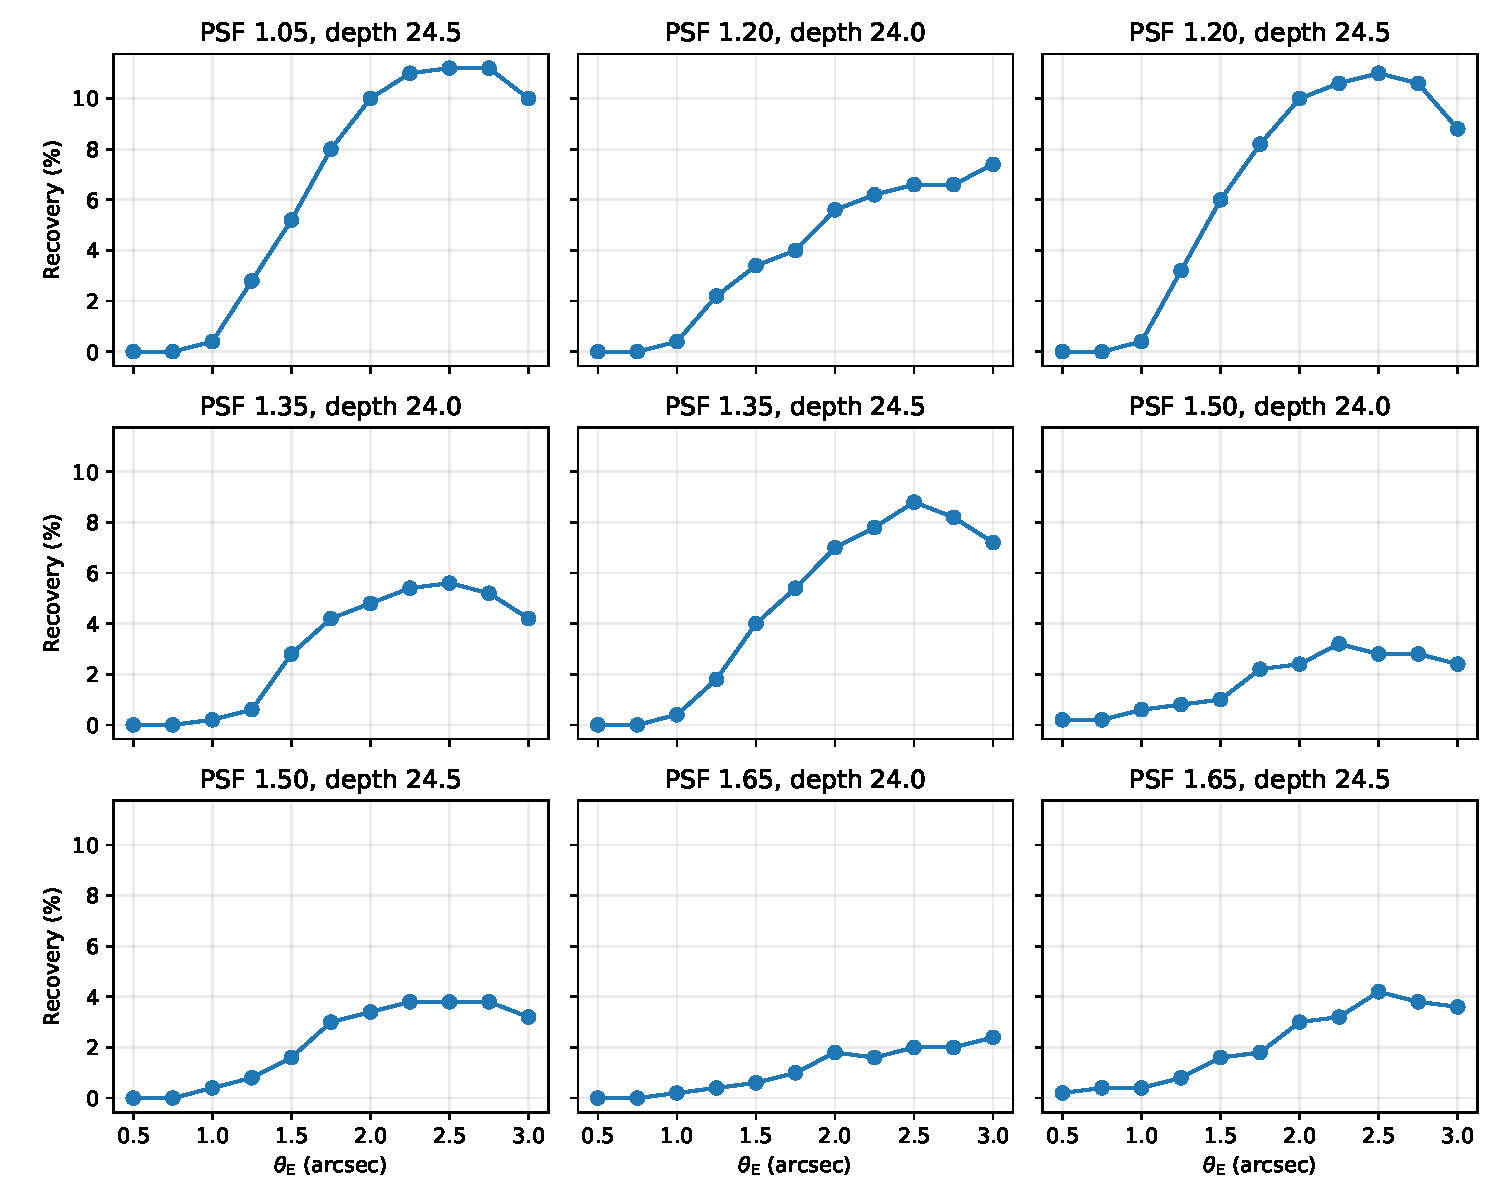
\includegraphics[width=\textwidth]{figures/appendix_grec_cell_radius_response.pdf}
\caption{Conditional \(G_{\rm rec}\) recovery versus Einstein radius in each
occupied PSF--depth cell. Every point contains 500 targets. The panels are
descriptive support strata covering nine of the ten possible PSF--depth
combinations.}
\label{fig:cell_radius_response}
\par\smallskip{\raggedright\noindent\textit{Alt text:} Nine panels show
recovery curves over eleven Einstein radii for the occupied combinations of
five PSF values and two depth values. The PSF 1.05, depth 24.0 combination is
absent from the design.\par}
\end{figure*}

\subsection{Fixed-target brightness and source-photon response}
\label{app:bounded_controls}

The brightness control contains 344 target--magnitude cells, 344 expectation
images, and 2,752 photon realizations. Table~\ref{tab:brightness_control}
reports equal-target recovery; photon rates first average eight draws within
target. Eight-draw finite-photon MCSE is at most 1.071 percentage points. Zero MCSE at
the faint nodes reflects eight all-negative draw-specific cohort rates, not a
general precision guarantee.

\begin{figure*}
\refstepcounter{table}\label{tab:brightness_control}
\noindent\textbf{Table~\thetable.} Fixed-target \(C_{\rm bright}\) recovery
percentages under the trained preprocessing and common threshold.
\begin{center}
\begin{tabular}{rrr}
\toprule
\(m_{r,\mathrm{src}}\) & Expectation & Photon \\
\midrule
18.5 & 13.953 & 12.500 \\
19.5 & 16.279 & 13.081 \\
20.5 & 18.605 & 18.314 \\
21.5 & 11.628 & 13.953 \\
22.5 & 9.302 & 7.558 \\
23.5 & 2.326 & 1.744 \\
24.5 & 0.000 & 0.000 \\
25.5 & 0.000 & 0.000 \\
\bottomrule
\end{tabular}
\end{center}
\medskip
\centering
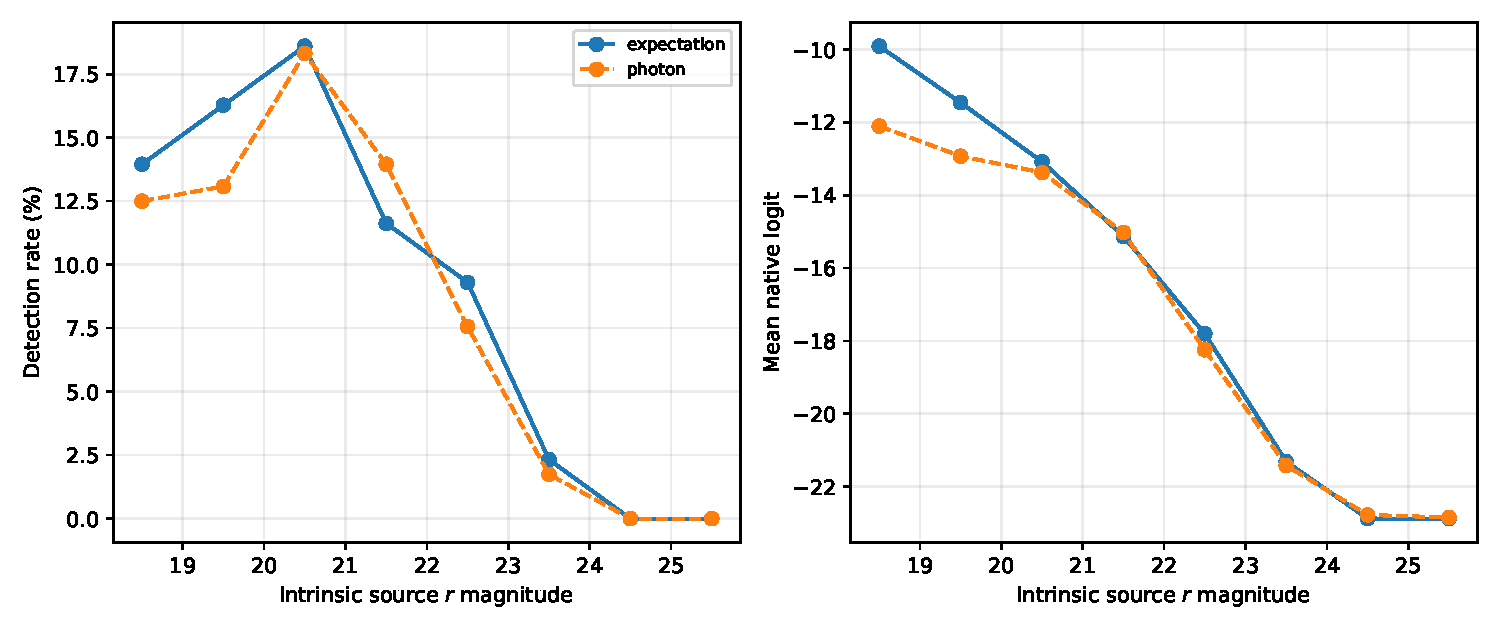
\includegraphics[width=0.9\textwidth]{figures/appendix_brightness_response.pdf}
\caption{Detection fraction and mean native logit versus intrinsic source
magnitude for the fixed 43-target brightness experiment. Expectation and
photon-realized images use the trained preprocessing and common threshold.
The detection fraction peaks near magnitude 20.5, whereas the mean logit
declines across the tested magnitude range. These are finite-cohort response
summaries on 43 fixed targets.}
\label{fig:brightness_response}
\par\smallskip{\raggedright\noindent\textit{Alt text:} Two panels show
expectation and photon-realized images over intrinsic source magnitudes 18.5
to 25.5. Detection fractions reach their maximum at 20.5 and are zero at 24.5
and 25.5. Mean logits decline toward fainter magnitudes. The photon and
expectation curves are close but not identical.\par}
\end{figure*}

This finite-cohort detector-response test characterizes the fixed targets and
tested source scalings; intrinsic magnitude supplies the controlled axis.
\FloatBarrier
\clearpage

\subsection{\(P_{\rm noise}\) draw-count pilot}
\label{app:pnoise_draw_pilot}

\noindent\begin{minipage}{\columnwidth}
The score-blind pilot contains 288 targets and 3,168 scenes, with 64 draws per
scene. MCSE and the target-sampling standard error are on the probability scale;
the latter is 0.003553. A candidate passes when MCSE is at most 0.002 and at
most 20 per cent of the target-sampling standard error. One draw is diagnostic
only because its MCSE is unavailable; eight is the smallest count satisfying
both criteria.

\begin{center}
\refstepcounter{table}\label{tab:pnoise_draw_pilot}
\noindent\textbf{Table~\thetable.} \(P_{\rm noise}\) design-pilot
photon-draw selection.
\par\smallskip
\scriptsize
\begin{tabular}{rcccc}
\toprule
Draws & MCSE & MCSE/SE & Absolute criterion & Relative criterion \\
\midrule
1  & unavailable & unavailable & No & No \\
2  & 0.001119 & 0.315 & Yes & No \\
4  & 0.000791 & 0.223 & Yes & No \\
\textbf{8}  & \textbf{0.000559} & \textbf{0.157} & \textbf{Yes} & \textbf{Yes} \\
16 & 0.000396 & 0.111 & Yes & Yes \\
32 & 0.000280 & 0.079 & Yes & Yes \\
64 & 0.000198 & 0.056 & Yes & Yes \\
\bottomrule
\end{tabular}
\end{center}
\end{minipage}

\subsection{Detector-checkpoint sensitivity}
\label{app:checkpoint_sensitivity}

Tables~\ref{tab:checkpoint_panel_endpoints} and
\ref{tab:checkpoint_panel_interventions} report the runs defined in
Section~\ref{sec:checkpoint_panel_design}, selected and calibrated as in
Section~\ref{sec:checkpoint_sensitivity_methods}. The within-run selection
metric is average precision from float32 sigmoid outputs on that run's
noisy-label validation population; an exact tie retains the earliest epoch.
The primary detector remains the terminal epoch-160 checkpoint.

\begin{table*}
\refstepcounter{table}\label{tab:checkpoint_panel_endpoints}
\noindent\textbf{Table~\thetable.} Final checkpoint-sensitivity endpoints.
Each \(t_m\) yields exactly 20 threshold exceedances among the same 20,002
calibration negatives. Achieved-FPR counts use the same 12,512-row evaluation
cohort; their percentages and the \(G_{\rm rec}\) percentages are followed by
95 per cent spatial-group intervals. Selected-system entries are exact counts
among the same 43 systems. Baseline denotes natural-prevalence sampling with
cosine scheduling; the other variant labels name the one changed training
factor. ``Both sources'' uses reviewed and additional catalogue candidates;
``Reviewed only'' omits the additional candidates. Validation AP is the
within-run checkpoint-selection value; values for the two positive-example
compositions are computed on validation populations with 778 and 64 noisy
positive labels, respectively, and should not be compared as if their labels
or prevalence were the same. The target FPR is an empirical calibration rate
rather than a guaranteed population rate.
\begin{center}
\scriptsize
\begin{tabular}{L{0.09\textwidth}L{0.07\textwidth}r r r r
                L{0.205\textwidth}r L{0.20\textwidth}}
\toprule
Variant & Positive examples & Seed & Epoch & Val.\ AP & \(t_m\) &
Achieved FPR: count; per cent [interval] & Selected &
\(G_{\rm rec}\): per cent [interval] \\
\midrule
Baseline & Both sources & 42 & 19 & 0.8104 & 1.153126 &
11; 0.0879 [0.0434, 0.1454] & 35/43 & 2.5717 [2.2801, 2.8757] \\
Baseline & Both sources & 123 & 17 & 0.8181 & 0.621170 &
13; 0.1039 [0.0550, 0.1656] & 37/43 & 2.4263 [2.1344, 2.7286] \\
Baseline & Both sources & 2026 & 93 & 0.8053 & 3.659930 &
16; 0.1279 [0.0738, 0.1948] & 37/43 & 3.1535 [2.8163, 3.5084] \\
\addlinespace
Baseline & Reviewed only & 42 & 103 & 0.7764 & -9.486459 &
17; 0.1359 [0.0773, 0.2093] & 37/43 & 1.8485 [1.6015, 2.1177] \\
Baseline & Reviewed only & 123 & 93 & 0.7704 & -8.606620 &
21; 0.1678 [0.1047, 0.2454] & 36/43 & 1.4525 [1.2305, 1.6973] \\
Baseline & Reviewed only & 2026 & 43 & 0.7679 & -1.618260 &
16; 0.1279 [0.0700, 0.2059] & 36/43 & 1.2808 [1.0801, 1.4987] \\
\addlinespace
50:50 sampler & Both sources & 42 & 62 & 0.7922 & 6.281433 &
12; 0.0959 [0.0502, 0.1552] & 35/43 & 2.8081 [2.4995, 3.1276] \\
50:50 sampler & Reviewed only & 42 & 37 & 0.7704 & -7.143696 &
17; 0.1359 [0.0751, 0.2150] & 37/43 & 1.3778 [1.1665, 1.6091] \\
\addlinespace
Step schedule & Both sources & 42 & 18 & 0.8109 & 1.875446 &
9; 0.0719 [0.0333, 0.1255] & 35/43 & 2.1071 [1.8303, 2.3978] \\
Step schedule & Reviewed only & 42 & 87 & 0.7653 & -2.322129 &
14; 0.1119 [0.0620, 0.1777] & 35/43 & 1.3636 [1.1628, 1.5833] \\
\addlinespace
Additional seed & Reviewed only & 7 & 86 & 0.7516 & -7.043954 &
14; 0.1119 [0.0611, 0.1763] & 39/43 & 1.3980 [1.1897, 1.6259] \\
Additional seed & Reviewed only & 2027 & 99 & 0.7695 & -9.008804 &
19; 0.1519 [0.0872, 0.2345] & 36/43 & 1.4040 [1.1922, 1.6399] \\
\bottomrule
\end{tabular}
\end{center}
\end{table*}

\medskip
\begin{table*}
\refstepcounter{table}\label{tab:checkpoint_panel_interventions}
\noindent\textbf{Table~\thetable.} Final checkpoint sensitivity of the paired
interventions. \(P_{\rm noise}\) is
modelled-photon-minus-expectation and
\(P_{\rm src}\) is S\'{e}rsic-minus-structured. Every row uses its
checkpoint-specific threshold yielding exactly 20 exceedances among 20,002
calibration negatives.
Estimates, intervals, and MCSE values are percentage points. The 95 per cent
intervals use one global target-spatial-group multiplier for
\(P_{\rm noise}\). For \(P_{\rm src}\), each pair receives the product of
global target-spatial and source multipliers, with source multipliers
normalised within the 16 source strata. MCSE uses the eight photon draws.
Baseline denotes natural-prevalence sampling with cosine scheduling; the
other variant labels name the one changed training factor. ``Both sources''
uses reviewed and additional catalogue candidates; ``Reviewed only'' omits
the additional candidates.
Intervals condition on the displayed checkpoint-specific thresholds and omit
calibration-sample variation.
\begin{center}
\scriptsize
\begin{tabular}{L{0.095\textwidth}L{0.075\textwidth}r r
                L{0.23\textwidth}r L{0.23\textwidth}r}
\toprule
Variant & Positive examples & Seed & Epoch &
\(P_{\rm noise}\) [95\% interval] & MCSE &
\(P_{\rm src}\) [95\% interval] & MCSE \\
\midrule
Baseline & Both sources & 42 & 19 & -0.9679 [-1.1321, -0.8137] & 0.0122 &
+0.3946 [+0.1622, +0.7152] & 0.0569 \\
Baseline & Both sources & 123 & 17 & -0.8379 [-0.9854, -0.7017] & 0.0120 &
+0.2683 [+0.0278, +0.5723] & 0.0207 \\
Baseline & Both sources & 2026 & 93 & -1.1644 [-1.3399, -0.9983] & 0.0130 &
+0.4261 [+0.1349, +0.8361] & 0.0651 \\
\addlinespace
Baseline & Reviewed only & 42 & 103 & -0.9672 [-1.1183, -0.8282] & 0.0088 &
+0.1184 [-0.0456, +0.3366] & 0.0303 \\
Baseline & Reviewed only & 123 & 93 & -0.7341 [-0.8719, -0.6123] & 0.0073 &
+0.0947 [-0.0411, +0.2952] & 0.0442 \\
Baseline & Reviewed only & 2026 & 43 & -0.7813 [-0.9180, -0.6529] & 0.0067 &
+0.0710 [-0.1679, +0.3166] & 0.0251 \\
\addlinespace
50:50 sampler & Both sources & 42 & 62 & -0.9982 [-1.1705, -0.8406] & 0.0129 &
+0.3946 [+0.1512, +0.7127] & 0.0752 \\
50:50 sampler & Reviewed only & 42 & 37 & -0.5111 [-0.6272, -0.4054] & 0.0091 &
+0.2446 [+0.0809, +0.5178] & 0.0469 \\
\addlinespace
Step schedule & Both sources & 42 & 18 & -0.7162 [-0.8697, -0.5764] & 0.0114 &
+0.3157 [+0.1297, +0.6001] & 0.0506 \\
Step schedule & Reviewed only & 42 & 87 & -0.8048 [-0.9429, -0.6789] & 0.0072 &
+0.1736 [+0.0530, +0.4061] & 0.0231 \\
\addlinespace
Additional seed & Reviewed only & 7 & 86 & -0.8535 [-1.0025, -0.7184] & 0.0073 &
+0.0947 [-0.0406, +0.2676] & 0.0207 \\
Additional seed & Reviewed only & 2027 & 99 & -0.7856 [-0.9292, -0.6546] & 0.0077 &
+0.0947 [-0.0740, +0.2794] & 0.0267 \\
\bottomrule
\end{tabular}
\end{center}
\end{table*}

The two-policy comparison, including designation of the validation-selected
policy for the main presentation, is exploratory. Under both policies all
12 aggregate \(P_{\rm noise}\) estimates are negative with intervals below
zero, and all 12 \(P_{\rm src}\) estimates are positive. Source-effect
intervals exclude zero for 7/12 validation-selected checkpoints and 8/12
terminal-epoch checkpoints. These related analyses describe policy
sensitivity within the same training runs.

A separate author-run
verification implementation reproduces the validation-selected epochs,
recorded checkpoint hashes, thresholds, row identities, estimates, intervals,
and MCSE values.

\subsection{Descriptive attribution of the pixel-statistic probe}

Using the same dependency-closed folds, component weights, and fold-local
standardisation, a secondary descriptive suite refits each of the 18
statistics alone and after its omission, and likewise evaluates each
photometric band. Median \(z\)-band pixel intensity is strongest: its
univariate OOF AUC is 0.888, omitting it reduces the multivariate AUC from
0.981 to 0.932, and its coefficient is positive in all five folds.
A \(z\)-band-only probe gives AUC 0.968 and omitting that band gives 0.929.
Here \(z\) denotes the band, not redshift. Median intensity can encode
foreground surface brightness, background level, or sample selection, so
the attribution summarizes a mixture of image-population properties. All 43
fits were separately recomputed by the authors as finite-cohort diagnostics.

\clearpage
\noindent\begin{minipage}{\columnwidth}
\subsection{\(G_{\rm rec}\) brightness stratifications}

Table~\ref{tab:grec_brightness} partitions the 49,500-scene grid and
1,710 detections by intrinsic source magnitude and by post-hoc source-only
in-stamp \(r\)-flux quartiles. Intrinsic magnitude is shared over the eleven
radii of a target, while one target can enter several rendered-flux quartiles.
Rates retain the original scene weights within bin. The bins are descriptive
intrinsic-magnitude and rendered-flux strata.

\begin{center}
\refstepcounter{table}\label{tab:grec_brightness}
\noindent\textbf{Table~\thetable.} Descriptive \(G_{\rm rec}\) brightness
stratifications at the primary threshold.
\par\smallskip
\resizebox{\columnwidth}{!}{%
\begin{tabular}{llrr}
\toprule
Stratification & Bin & Detections / scenes & Recovery (\%) \\
\midrule
Intrinsic \(m_{r,\mathrm{src}}\) & \([23,24)\) & 1,367 / 16,170 & 8.454 \\
Intrinsic \(m_{r,\mathrm{src}}\) & \([24,25)\) & 323 / 16,995 & 1.901 \\
Intrinsic \(m_{r,\mathrm{src}}\) & \([25,26)\) & 20 / 16,335 & 0.122 \\
\midrule
Rendered source \(r\)-flux & Lowest quartile & 11 / 12,375 & 0.089 \\
Rendered source \(r\)-flux & Second quartile & 7 / 12,375 & 0.057 \\
Rendered source \(r\)-flux & Third quartile & 241 / 12,375 & 1.947 \\
Rendered source \(r\)-flux & Highest quartile & 1,451 / 12,375 & 11.725 \\
\bottomrule
\end{tabular}
}
\end{center}
\end{minipage}

\subsection{Photon replay, normalization, and gain sensitivity}
\label{app:photon_followup}

The replay cohort contains 4,568 registered photon-draw realizations derived
from 571 deterministic expectation images and includes both score-blind
coverage and deliberately selected crossing cases. Replayed native score bits
agree with the retained scores for these realizations. Using each deterministic
expectation image's annular normalization statistics instead of recalculating
them for its photon-draw realization changes three decisions. Most selected
threshold changes therefore persist under expectation-anchored normalization.
This replay shows normalization sensitivity in the inspected cohort, but it
does not cover the complete photon bank.

\newpage
The separate gain diagnostic contains 198 scenes from 18 targets in 17
spatial groups. Deterministic recovery is 5/198, or 2.5253 per cent. Sixteen
keyed draws per scene give Table~\ref{tab:gain_followup}. The registered eight
gain-150 draws on these same scenes give 39/1,584, or 2.4621 per cent,
compared with 2.4937 per cent in the 16-draw gain-150 sample. This agreement on
common scene support shows that the gain comparison applies only to these 198
scenes and should not be compared directly with the full-grid estimate.

\medskip
\refstepcounter{table}\label{tab:gain_followup}
\noindent\textbf{Table~\thetable.} Fixed-cohort gain sensitivity. Changes are
relative to deterministic expectation. Gain is in
\({\rm e^{-}\,nmgy^{-1}}\); change and MCSE are percentage points. MCSE is
conditional photon Monte Carlo error, not a target-population interval.
\begin{center}
\small
\begin{tabular}{rrrr}
\toprule
Gain & Positive / 3,168 & Recovery (\%) & Change / MCSE \\
\midrule
75  & 59 & 1.8624 & \(-0.6629\) / 0.1961 \\
150 & 79 & 2.4937 & \(-0.0316\) / 0.1813 \\
300 & 82 & 2.5884 & \(+0.0631\) / 0.1299 \\
600 & 86 & 2.7146 & \(+0.1894\) / 0.1044 \\
\bottomrule
\end{tabular}
\end{center}

\subsection{Author-run endpoint and experiment checks}

Table~\ref{tab:independent_checks} distinguishes checks of the external and
operational feature protocols from checks of the thresholded experiments.
The checks separately verify feature extraction, classifier-head
reconstruction, out-of-fold calculations, and estimator refitting from the
archived arrays. Numerical agreement is evaluated under the recorded software
versions and backend.

Exactly 39/43 selected systems exceed the primary threshold. A separate
author-run implementation rehashes the 43 payload arrays and reproduces the
native score bits, decisions, and result. The endpoint is the response of
this finite cohort; no population interval is attached.

Figure~\ref{fig:missed_selected_systems} shows all four non-detections rather
than a selected subset, under one common display mapping.

Per-scene convergence diagnostics are absent from the final manifest for
43,780 stored \(G_{\rm rec}\) deterministic expectation images. For 2,364 of
those retained rows, the diagnostics remain in their bound generating
manifest; 41,416 rows lack diagnostics in both supplied manifests. Numerical
qualification therefore also uses the specified 142-scene reconstruction
audit. One scene required order-48 quadrature; its identity and image checksum
are recorded. For rows without diagnostics, the reconstructed manifest order
field is not treated as a per-scene convergence record.

\begin{table*}
\refstepcounter{table}\label{tab:independent_checks}
\noindent\textbf{Table~\thetable.} Author-run checks of the reported
experiment products. OOF denotes out-of-fold.
\begin{center}
\small
\begin{tabular}{L{0.13\textwidth}L{0.22\textwidth}L{0.58\textwidth}}
\toprule
Analysis & Verified support & Author-run check \\
\midrule
\(G_{\rm rec}\) &
49,500 rows; 4,500 targets; 2,187 spatial groups &
MPS logits and score bindings were reproduced; both 10,000-draw multiplier
calculations agreed. \\
\(G_{\rm domain}\), external/elementary &
6,379 rows; 561 dependency components &
Same-version refits from each persisted final matrix reproduce every OOF
score exactly under the recorded folds, weights, scaler, and estimator. \\
\(G_{\rm domain}\), operational &
6,379 rows; 1,280 features per row &
The retained head reconstructs all 6,379 native logits bit for bit on the
recorded MPS backend, and the same-version OOF refit is exact. \\
\(G_{\rm match}\), external/elementary &
129 rows; 43 triplets; 43 dependency components &
Current row identities, dependency closure, pair movements, and shared-axis
AUC arithmetic were recomputed from the persisted final axis scores. This
check recomputes the statistics from archived axis scores but does not repeat
feature extraction. \\
\(G_{\rm match}\), operational &
129 rows; 43 triplets; 43 dependency components &
Pair movements and shared-axis AUC arithmetic were recomputed from persisted
final axis scores; this is an arithmetic check rather than an independent
feature extraction. \\
\(P_{\rm noise}\) &
49,500 deterministic expectations; 396,000 photon-draw realizations &
The complete stored score table, primary point estimate, interval, and
finite-draw MCSE were recomputed. The separate 4,568-row replay in
Appendix~\ref{app:photon_followup} is a fixed implementation diagnostic. \\
\(P_{\rm src}\) &
1,584 pairs; 12,672 pair-draw rows &
All 1,584 photon artefacts were rehashed; native score bits and decisions,
pair averages, point estimate, interval, and finite-draw MCSE were separately
recomputed. \\
\bottomrule
\end{tabular}
\end{center}
\end{table*}

\medskip
\begin{figure*}
\begin{center}
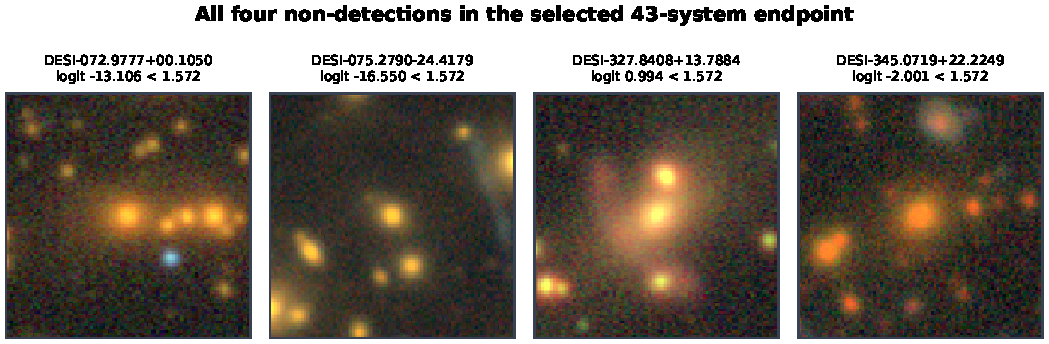
\includegraphics[width=0.82\textwidth]{figures/appendix_missed_selected_systems.pdf}
\end{center}
\refstepcounter{figure}\label{fig:missed_selected_systems}
\noindent\textbf{Figure~\thefigure.} All four non-detections among the 43
selected confirmed systems at
the primary threshold \(t_{10^{-3}}=1.5717214346\). Titles give the catalogue
name and native-float32 logit. Every panel uses the same complete
\(101\times101\)-pixel Legacy Survey \(z/r/g\) display mapping defined in
Equation~\ref{eq:rgb_preprocessing}; no panel-specific intensity rescaling or
crop is applied. The figure shows all four missed systems, not a
representative sample of the 43-system cohort.
\par\smallskip{\raggedright\noindent\textit{Alt text:} Four square Legacy Survey colour
cutouts arranged in one row. Each title identifies a confirmed system and
shows its logit below the common threshold. The images contain bright
foreground objects and surrounding structures with varied colour and
configuration.\par}
\medskip
\end{figure*}
\FloatBarrier

\subsection{Object-level provenance of the 43-system endpoint}

\label{app:confirmed_provenance}
The selected endpoint is not a uniformly dual-spectroscopic
sample. Table~\ref{tab:confirmed_43_provenance}
lists the object identifier, confirmation route, principal
object-level publication, and one representative recorded
foreground and source redshift for every evaluated system.
Multiple measurements and the complete evidence record are provided in
\texttt{confirmed\_43\_provenance.csv} in the reproducibility materials;
``--'' means that no
representative role-assigned redshift is recorded. The
confirmation-route column identifies whether displayed values
are secure, probable, low-confidence, or unverified.

\begin{table*}
\centering
\caption{Object-level provenance of the selected 43-system endpoint.}
\label{tab:confirmed_43_provenance}
{\scriptsize
\setlength{\tabcolsep}{3pt}
\renewcommand{\arraystretch}{0.92}
\begin{tabular}{p{0.14\textwidth}p{0.28\textwidth}p{0.24\textwidth}rr}
\toprule
Identifier & Confirmation route & Principal evidence & $z_{\rm foreground}$ & $z_{\rm source}$ \\
\midrule
\texttt{0361p000\_6437} & secure foreground and source spectra & \citep{Gladders2002,Gladders2003} & 0.773 & 4.8786 \\
\texttt{0442m235\_7484} & secure foreground and source spectra & \citep{Zitrin2011,Nakane2025} & 0.5049 & 1.09 \\
\texttt{0537m132\_1571} & secure foreground and source spectra & \citep{Lin2026} & 0.3866 & 2.30117 \\
\texttt{0572m102\_2469} & secure foreground and source spectra & \citep{Lin2026} & 0.74493 & 1.60376 \\
\texttt{0656m280\_3774} & secure foreground and source spectra & \citep{Lin2026} & 0.62107 & 1.17482 \\
\texttt{0728p000\_6851} & secure source; foreground spectrum unverified & \citep{Sand2005} & 0.430 & 2.007 \\
\texttt{0734m102\_4599} & secure foreground and source spectra & \citep{Richard2010,Lin2026} & 0.24820 & 1.043 \\
\texttt{0750m307\_2398} & secure foreground and source spectra & \citep{Lin2026} & 0.44137 & 1.44884 \\
\texttt{0753m245\_3999} & secure foreground and source spectra & \citep{Lin2026} & 0.32059 & 2.8290 \\
\texttt{0862m265\_8849} & secure foreground and source spectra & \citep{Lin2026} & 0.27534 & 2.17441 \\
\texttt{0870m362\_8874} & secure foreground and source spectra & \citep{Lin2026} & 0.3011 & 0.84611 \\
\texttt{0910m360\_2444} & secure foreground and source spectra & \citep{Lin2026} & 0.4883 & 1.43211 \\
\texttt{1219p105\_7293} & secure foreground and source spectra & \citep{Huang2026,Lin2026,Tran2022} & 0.475 & 1.23742 \\
\texttt{1409p185\_769} & secure foreground and source spectra & \citep{Huang2026,Tran2022} & 0.873 & 2.41673 \\
\texttt{1434p092\_2623} & secure lens; probable source spectrum & \citep{Tran2022} & 0.743 & 2.43243 \\
\texttt{1601p187\_3957} & secure foreground and source spectra & \citep{Lin2026,Tran2022} & 0.314 & 0.87872 \\
\texttt{1614m087\_3206} & secure lens; low-confidence source spectrum & \citep{Lin2026} & 0.82754 & 2.079 \\
\texttt{1655m060\_944} & secure foreground and source spectra & \citep{Zaborowski2023,Huang2026} & 0.4834 & 1.67511 \\
\texttt{1658p122\_150} & imaging/model; no secure dual spectra & \citep{Huang2026} & -- & -- \\
\texttt{1671p042\_499} & secure foreground and source spectra & \citep{Lin2026} & 0.35153 & 1.28023 \\
\texttt{1683p240\_1137} & secure foreground and source spectra & \citep{Kubo2009} & 0.3361 & 0.766 \\
\texttt{1686p167\_5461} & secure foreground and source spectra & \citep{Stark2013,Lin2026} & 0.537 & 1.718 \\
\texttt{1744p147\_5445} & secure foreground and source spectra & \citep{Lin2026} & 0.56486 & 2.41864 \\
\texttt{1894p150\_8726} & secure foreground and source spectra & \citep{Huang2026,Tran2022} & 0.57160 & 1.16149 \\
\texttt{1908p212\_1676} & secure foreground and source spectra & \citep{Lin2026} & 0.34832 & 1.48152 \\
\texttt{1928p017\_9908} & imaging/model; no secure dual spectra & \citep{Huang2026} & -- & -- \\
\texttt{1976p147\_245} & secure foreground and source spectra & \citep{Lin2026} & 0.26144 & 0.85834 \\
\texttt{2006p037\_9179} & secure foreground and source spectra & \citep{Lin2026,Tran2022} & 0.353 & 1.01590 \\
\texttt{2026p047\_4274} & secure foreground and source spectra & \citep{Huang2026,Lin2026,Tran2022} & 0.336 & 1.16757 \\
\texttt{2168m067\_3815} & secure foreground and source spectra & \citep{Zaborowski2023,Tran2022} & 0.26500 & 1.51409 \\
\texttt{2204p147\_3771} & secure foreground and source spectra & \citep{Stark2013,Pettini2010} & 0.741 & 1.433 \\
\texttt{2276p205\_1624} & imaging/model; no secure dual spectra & \citep{Huang2026} & -- & -- \\
\texttt{2349p167\_2044} & secure foreground and source spectra & \citep{Huang2026,Tran2022,Barone2026} & 0.409 & 1.833 \\
\texttt{2530p280\_351} & imaging/model; no secure dual spectra & \citep{Huang2026} & -- & -- \\
\texttt{2608p237\_3728} & secure foreground and source spectra & \citep{Lin2026} & 0.2296 & 0.97503 \\
\texttt{3108m062\_2639} & secure foreground and source spectra & \citep{Huang2026,Tran2022,Barone2026} & 0.79261 & 1.892 \\
\texttt{3277p137\_6699} & secure lens; probable source spectrum & \citep{Huang2026,Tran2022,Barone2026} & 0.20643 & 0.890 \\
\texttt{3409p280\_5325} & secure foreground and source spectra & \citep{Lin2026,Tran2022} & 0.343 & 0.96034 \\
\texttt{3418m020\_1357} & secure foreground and source spectra & \citep{Lin2026,Sand2005} & 0.330 & 2.237 \\
\texttt{3428m035\_4814} & secure foreground and source spectra & \citep{Lin2026} & 0.24592 & 1.05956 \\
\texttt{3431m042\_1867} & secure lens; low-confidence source spectrum & \citep{Lin2026} & 0.43519 & 0.58 \\
\texttt{3450p222\_3227} & secure foreground and source spectra & \citep{Wen2011,Stark2013} & 0.443 & 1.93 \\
\texttt{3459p235\_481} & secure foreground and source spectra & \citep{Lin2026} & 0.27653 & 1.29593 \\
\bottomrule
\end{tabular}
}
\end{table*}

\FloatBarrier

\subsection{Injection-target and matching support}

The 4,500 \(G_{\rm rec}\) targets are catalogue-selected injection targets, not
confirmed deflectors. Their Tractor types are 2,853 SER, 1,213 DEV, and 434
REX. Observed \(z\) magnitude has median 19.40, interquartile range
18.71--19.77, and range 13.29--20.00. The
selection manifest contains no homogeneous catalogue photo-\(z\) field for
these 4,500 rows. Photo-\(z\), velocity dispersion, stellar mass, and
environment therefore neither select these targets nor assign their SIE
parameters.

Under the score-blind assignment in Section~\ref{sec:decomposition_methods},
all 43 references receive unique targets. There are 168--4,229 admissible
targets per reference, and selected robust-IQR distances range from 0.108 to
1.140. Table~\ref{tab:gmatch_coverage} reports the measured support before
and after matching.

Direct checks of the stored bare and injected arrays verified their pairing
and the recorded target, source, lens, PSF, rendering, random, and flux
identities. No target-total flux floor, post-lensing flux rescaling, detector
score, or probe outcome enters matching or pair construction. The matching
set covers five measured image and catalogue quantities; homogeneous
deflector redshift, mass, environment, and observed-source brightness are
unavailable across all references.

\medskip
\noindent\begin{minipage}{\columnwidth}
\refstepcounter{table}\label{tab:gmatch_coverage}
\noindent\textbf{Table~\thetable.} Measured-covariate support for the 43
references, complete
\(G_{\rm rec}\) target roster, and 43 matched targets. Entries give
minimum/median/maximum; redshift, mass, environment, and source properties are
outside the matching set.
\begin{center}
\scriptsize
\resizebox{\columnwidth}{!}{%
\begin{tabular}{lrrr}
\toprule
Covariate & References & Target roster & Matched targets \\
\midrule
Observed \(z\) magnitude & 15.71/17.11/21.08 & 13.29/19.40/20.00 &
15.67/17.07/19.97 \\
S\'{e}rsic index & 1.00/4.34/6.00 & 0.50/2.60/6.00 &
0.66/4.27/6.00 \\
Axis ratio & 0.15/0.70/0.95 & 0.052/0.61/1.00 &
0.20/0.70/0.93 \\
\(r\)-band PSF FWHM (arcsec) & 1.01/1.27/1.81 & 0.98/1.39/1.72 &
1.00/1.27/1.70 \\
\(r\)-band depth (mag) & 24.10/24.47/25.75 & 23.79/24.30/26.44 &
24.10/24.41/25.65 \\
\bottomrule
\end{tabular}
}
\end{center}
\end{minipage}

\subsection{\(P_{\rm src}\) source construction and design}

For the regularised COSMOS F814W source construction defined in
Section~\ref{sec:source_models} \citep{Mandelbaum2012}, we report the realised
map-quality diagnostics and draw-count pilot below.

Of 81,499 catalogue rows, 770 satisfy the source criteria and 144 are
selected without detector outcomes for the final experiment. The maximum
structured--S\'{e}rsic centroid separation after construction is
\(7.34\times10^{-5}\) arcsec, the minimum retained positive-flux fractions
are 0.9010 and 0.9561 for the structured and S\'{e}rsic arms, respectively,
and their source-map pixel correlations range from 0.6190 to 0.9985
(median 0.9767). These diagnostics characterise construction fidelity; they
span visibly similar and dissimilar source-map pairs within the design.

A separate pilot used 1,584 pairs formed from 144 targets and 144 sources that
do not appear in the final experiment. Its joint distribution over the nine
target cells, eleven Einstein radii, and sixteen source strata is identical to
the final design. The pilot and final samples are disjoint in pair, underlying-scene,
target, spatial, physical, coordinate, pixel-hash, source, map-hash, and
ancestry fields. The number of photon draws was chosen before the final
experiment was scored.

The pilot scores 64 photon draws per pair. Table~\ref{tab:psrc_draw_pilot}
shows the empirical MCSE at each candidate count. The selection
rule chooses the smallest passing count, so eight draws are selected before
final scoring.

\medskip
\noindent\begin{minipage}{\columnwidth}
\refstepcounter{table}\label{tab:psrc_draw_pilot}
\noindent\textbf{Table~\thetable.} \(P_{\rm src}\) design-pilot photon-draw
selection. MCSE values and the target 0.01 are on the probability
scale; 0.01 equals one percentage point. Eight is the smallest
candidate count.
\begin{center}
\begin{tabular}{rrc}
\toprule
Draws & Measured MCSE & Pass \\
\midrule
8  & 0.000683 & Yes \\
16 & 0.000633 & Yes \\
32 & 0.000387 & Yes \\
64 & 0.000255 & Yes \\
\bottomrule
\end{tabular}
\end{center}
\end{minipage}


The final design contains 1,584 distinct targets in 1,219 spatial groups,
with the 99 target-cell--radius blocks and balanced source reuse specified in
Section~\ref{sec:paired_source_construction}.
Section~\ref{sec:paired_source_estimators} defines the corresponding weighting
and multiway uncertainty.

Before photon draws or detector scoring, all 1,584 paired expectation images
pass the convergence comparison at oversampling factors 4, 8, and
16. The maximum consecutive relative \(L_1\) difference is 0.002212, below
the 0.01 criterion. The eight selected photon draws then produce 12,672 pair-draw
rows per arm for the estimate reported in
Section~\ref{sec:paired_source_results}.

Under the reduced-cohort equal-cell rule, leave-one-source-out estimates range
from \(+0.524813\) to \(+0.580140\) percentage points, and
leave-one-spatial-group estimates range from \(+0.521104\) to \(+0.576299\)
points. No deletion changes the
sign. These are influence diagnostics rather than additional confidence
intervals.

\subsection{Noiseless known-source transfer}
\label{app:source_transfer_followup}

We tested the preparation route with 16 noiseless known-source cases covering
the retained source strata. Against an independently spatially refined
analytic reference, the maximum normalized \(L_1\) discrepancy is 0.08335 per
cent and the maximum production centroid residual is
\(3.72\times10^{-5}\) arcsec. All cases meet the global-\(L_1\),
centring, and normalization adequacy criteria, using limits of 1 per cent and
\(3\times10^{-4}\) arcsec for the first two quantities. Under the stricter
diagnostics, the local-pixel criterion is met in 1/16 cases and the shape
criterion in 0/16. The global and stricter summaries therefore characterize
different aspects of the same 16-case numerical check.

\subsection{Renderer reconciliation}
\label{app:renderer_reconciliation}

The renderer test contains 142 scenes: the 43 matched-design injections, the
order-48 scene, and one scene from each cell--radius stratum, with one overlap
among these groups. This sample tests numerical implementation across the
design but does not cover every production scene.
Every scene passes replay and production quadrature convergence,
independent optical-reference convergence after deterministic refinement
where required, comparison with an effective post-pixel Gaussian reference,
and comparison of production-support SIE deflections with an independent
implementation.
The effective-PSF comparison jointly changes operation order and FFT boundary
handling and therefore tests their combined implementation.

The maximum and 95th-percentile production/reference relative \(L_1\)
differences are 0.007695 and 0.005802. The maximum centroid difference is
0.02293 native pixel, the minimum pixel correlation is 0.999952, and the
maximum production-support SIE vector error is
\(9.06\times10^{-9}\) arcsec. These bounds summarize numerical agreement for
the audited scenes within the tested support.

The softened near-circular branch occurs in zero of the 49,500
realised \(G_{\rm rec}\) scenes and zero of the 1,584 \(P_{\rm src}\) pairs.
Production-support SIE tests pass; the separate boundary-specific test does
not meet its predefined criterion.

\vspace{-2pt}
\FloatBarrier


\end{document}
